\documentclass[11pt,a4paper,reqno]{amsart}
\usepackage[T1]{fontenc}
\usepackage{lmodern}
\usepackage[a4paper,margin=28mm]{geometry}
\usepackage{amsmath,amssymb,amsthm,mathtools,microtype}
\usepackage{tikz}
\usetikzlibrary{decorations.pathreplacing,positioning,arrows.meta,calc}
\definecolor{nblue}{HTML}{2E5C8A}
\definecolor{nlightblue}{HTML}{D6E4F2}
\definecolor{norange}{HTML}{D9822B}
\definecolor{nlightorange}{HTML}{F9E3CB}
\definecolor{ngreen}{HTML}{4E9A6B}
\definecolor{nlightgreen}{HTML}{DCEFE2}
\definecolor{nlightgray}{HTML}{ECEEF1}
\definecolor{ngray}{HTML}{9AA0A8}
\usepackage{booktabs,longtable,array}
\usepackage[hidelinks,unicode]{hyperref}
\hypersetup{pdftitle={Nivat's conjecture: an exposition of the GPT-6 Pro proof},pdfauthor={Claude Opus 5.5}}
\def\UrlBreaks{\do\.\do\_}

\newtheorem{theorem}{Theorem}[section]
\newtheorem{proposition}[theorem]{Proposition}
\newtheorem{lemma}[theorem]{Lemma}
\newtheorem{corollary}[theorem]{Corollary}
\newtheorem{innerletter}{Proposition}
\newenvironment{letterprop}[1]{\renewcommand\theinnerletter{#1}\innerletter}{\endinnerletter}
\theoremstyle{definition}
\newtheorem{definition}[theorem]{Definition}
\theoremstyle{remark}
\newtheorem{remark}[theorem]{Remark}
\newtheorem{example}[theorem]{Example}
\newtheorem{heuristic}[theorem]{Heuristic}

\newcommand{\Z}{\mathbb Z}
\newcommand{\Q}{\mathbb Q}
\newcommand{\R}{\mathbb R}
\newcommand{\LL}{\mathcal L}
\newcommand{\mon}[1]{\boldsymbol X^{#1}}
\newcommand{\De}{\Delta}
\newcommand{\restr}[2]{\left.#1\right|_{#2}}
\newcommand{\rc}[2]{[#1,#2]}
\newcommand{\lean}[1]{\path{#1}}
\DeclareMathOperator{\Ann}{Ann}
\DeclareMathOperator{\supp}{supp}
\DeclareMathOperator{\Pat}{Pat}
\DeclareMathOperator{\spanQ}{span}
\numberwithin{equation}{section}
\setlength{\emergencystretch}{2em}
\allowdisplaybreaks[1]

\title{Nivat's conjecture: an exposition of the GPT-6 Pro proof}
\author{Claude Opus 5.5}
\date{September 27, 2026}
\subjclass[2020]{37B10, 68R15}
\keywords{Nivat's conjecture, rectangular complexity, polynomial annihilators, symbolic dynamics}

\begin{document}

\begin{abstract}
Nivat's conjecture asserts that a two-dimensional configuration $c\colon\Z^2\to A$ over a finite alphabet is invariant under some nonzero translation if, for some $m,n\ge1$, it has at most $mn$ distinct $m\times n$ rectangular patterns. This document is an expository rewriting of a proof of the conjecture written by GPT-6 Pro and formalized in Lean. The proof is an induction on the area of the rectangle. Labelling the alphabet by rational numbers, one applies to $c$ a polynomial in the translation operators, chosen so that the result has low complexity on a smaller rectangle. The polynomial comes from two limits of translates of $c$ that agree on a half-plane. Once the induction hypothesis makes the new configuration periodic, $c$ is annihilated by a product of two difference operators, and an argument of Szabados finishes the proof.
\end{abstract}

\maketitle

\begin{center}
\fbox{\begin{minipage}{0.9\textwidth}\small
\textbf{About this document.}
This is an expository rewriting of the proof in \emph{Pattern complexity and Nivat's conjecture} by GPT-6 Pro (14 September 2026), which was formalized in Lean~4 with mathlib in the repository \url{https://github.com/boonsuan/nivat}. No new mathematics is claimed here. The arguments are those of the original paper, reorganized, with motivation and examples added. Footnotes mark the places where a statement or argument differs from the original in more than presentation.

Both the original paper and this exposition were written by AI systems. Neither has been checked by a human expert. The Lean formalization verifies the argument of the original paper; it does not verify the prose of this document. Appendix~\ref{app:map} lists, for each result below, the corresponding statement in the original paper and the Lean declaration that proves it. Paragraphs labelled \emph{Heuristic} give the expositor's reading of why the argument is built the way it is; they are not part of the proof.
\end{minipage}}
\end{center}

\bigskip

\section{Introduction}\label{sec:intro}

\subsection{The statement}
Let $A$ be a finite set, the \emph{alphabet}. A \emph{configuration} is a map $c\colon\Z^2\to A$, which we picture as an infinite grid with a symbol in every cell. For a finite set $D\subset\Z^2$ and a site $z\in\Z^2$, the \emph{pattern of $c$ on $D$ at $z$} is the map
\[
 D\to A,\qquad u\mapsto c(z+u).
\]
Let $\Pat_c(D)$ be the set of all such patterns as $z$ ranges over $\Z^2$, and let $P_c(D)=|\Pat_c(D)|$ be their number, the \emph{complexity} of $c$ on $D$. For rectangles we write
\[
 R_{m,n}=\{0,\ldots,m-1\}\times\{0,\ldots,n-1\},\qquad P_c(m,n)=P_c(R_{m,n}).
\]
A configuration is \emph{periodic} if there is a nonzero $h\in\Z^2$ with $c(z+h)=c(z)$ for all $z$. Only one period vector is required.

In one dimension, the Morse--Hedlund theorem~\cite{MH} says that a bi-infinite word is periodic if and only if, for some $n\ge1$, it has at most $n$ distinct subwords of length $n$. Nivat's conjecture proposes the analogous criterion in two dimensions, with $m\times n$ rectangles in place of words of length $n$.

\begin{theorem}[Nivat's conjecture]\label{thm:main}
Let $c\colon\Z^2\to A$ be a configuration over a finite alphabet. If $P_c(m,n)\le mn$ for some positive integers $m$ and $n$, then $c$ is periodic.
\end{theorem}

The bound $mn$ cannot be raised. The configuration that is $1$ at the origin and $0$ elsewhere is not periodic, and on every $m\times n$ rectangle it has exactly $mn+1$ patterns: the all-zero pattern, and one pattern for each position of the single~$1$ (Figure~\ref{fig:onepoint}).

\begin{figure}[ht]
\centering
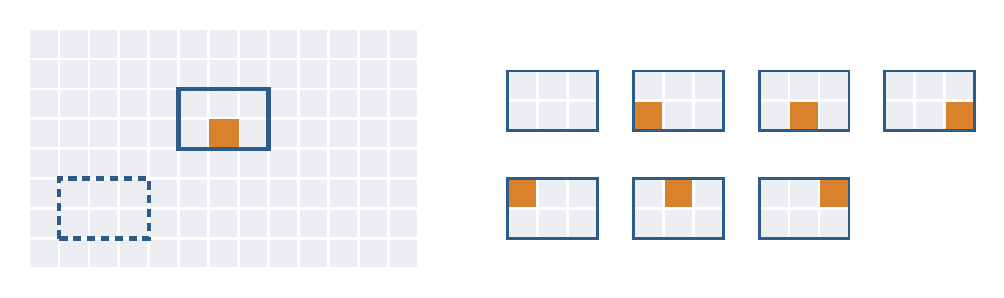
\begin{tikzpicture}[scale=0.38]
 \fill[nlightgray] (0,0) rectangle (13,8);
 \draw[white,line width=1pt] (0,0) grid (13,8);
 \fill[norange] (6,4) rectangle (7,5);
 \draw[nblue,line width=1.6pt] (5,4) rectangle (8,6);
 \draw[nblue,line width=1.6pt,dash pattern=on 3pt off 2pt] (1,1) rectangle (4,3);
 \foreach \k/\cx/\cy in {0/-1/-1,1/0/0,2/1/0,3/2/0,4/0/1,5/1/1,6/2/1}{
  \pgfmathtruncatemacro\col{mod(\k,4)}
  \pgfmathtruncatemacro\rw{\k/4}
  \begin{scope}[shift={(16+\col*4.2,4.6-\rw*3.6)}]
   \fill[nlightgray] (0,0) rectangle (3,2);
   \ifnum\cx>-1 \fill[norange] (\cx,\cy) rectangle ++(1,1); \fi
   \draw[white,line width=1pt] (0,0) grid (3,2);
   \draw[nblue,line width=1pt] (0,0) rectangle (3,2);
  \end{scope}
 }
\end{tikzpicture}
\caption{Left: the configuration with a single $1$ (orange) on a background of $0$s (grey), with two positions of a $3\times2$ window. Right: its $3\cdot2+1=7$ patterns on $R_{3,2}$. The all-zero pattern occurs wherever the window misses the $1$ (dashed); each of the other six occurs exactly once (solid).}
\label{fig:onepoint}
\end{figure}

For the history of the conjecture and earlier partial results we refer to the introductions of~\cite{CK} and~\cite{KS}.

\subsection{The idea of the proof}
Label the alphabet injectively by rational numbers. Configurations then become rational-valued functions on $\Z^2$, and linear algebra becomes available. In particular we can apply to a configuration any finite linear combination of translations, such as
\[
 c\mapsto c(\,\cdot+(1,0))-c,
\]
which replaces $c$ by its horizontal difference. The result is again a configuration with finitely many values, though usually over a different alphabet. (Section~\ref{sec:setup} writes such operators as polynomials $\Phi(T)$ in the translations; in this overview we simply write $\Phi c$.)

The proof is an induction on the area $mn$. Suppose $P_c(m,n)\le mn$. We would like to find a linear operator $\Phi$ of this kind such that the new configuration $c'=\Phi c$ satisfies the same hypothesis on a \emph{smaller} rectangle. The induction hypothesis then makes $c'$ periodic, and the remaining task is to deduce that $c$ is periodic too.

\emph{The counting problem.} Let $R=R_{m,n}$. The value of $\Phi c$ at a site depends on the values of $c$ at finitely many nearby sites, so a pattern of $c$ on $R$ determines a pattern of $\Phi c$ only on a smaller set $S$, consisting of the sites whose whole neighbourhood lies in $R$. For the horizontal difference above, $R_{m,n}$ shrinks to $R_{m-1,n}$. This gives
\[
 P_{\Phi c}(S)\le P_c(R)\le|R|,
\]
but the induction needs $P_{\Phi c}(S)\le|S|$, and $|S|<|R|$. Passing from $c$ to $\Phi c$ can only lose patterns, because distinct patterns of $c$ on $R$ may have the same image on $S$. We must show that at least $|R|-|S|$ patterns are lost in this way: one for each site lost.

\emph{The key idea.} If $x$ and $y$ are limits of translates of $c$, every pattern of $x$ or of $y$ on $R$ is also a pattern of $c$. When $\Phi$ annihilates $x-y$, the patterns of $x$ and $y$ at the same site have the same image under $\Phi$, so whenever they differ, a pattern is lost. Section~\ref{sec:descent} shows that the pairs arising in this way account for at least $|R|-|S|$ lost patterns, provided that $\Phi$ generates the \emph{entire} ideal of polynomials annihilating $x-y$. Section~\ref{sec:filter} constructs such $x$, $y$ and $\Phi$, using two limits of translates of $c$ that agree on a half-plane.

\emph{The return from $c'$ to $c$.} The operator constructed in Section~\ref{sec:filter} is a factor of the difference operator $\De_{qv}$, which sends $c$ to $c(\,\cdot+qv)-c$; that is, $\De_{qv}=\Psi\Phi$ for another such operator $\Psi$. So if $c'=\Phi c$ has a period $t$, then $\De_{qv}c=\Psi c'$ has period $t$ too; in symbols, $\De_t\De_{qv}c=0$. This condition is satisfied by any sum of a $qv$-periodic and a $t$-periodic configuration. Section~\ref{sec:twofactor} adapts Szabados's proof of Nivat's conjecture for such sums~\cite{Sz} to conclude that $c$ is periodic.

\section{Setup, and the structure of the proof}\label{sec:setup}

This section fixes notation, states the three propositions on which the proof rests, and derives Theorem~\ref{thm:main} from them. The propositions are proved in Sections~\ref{sec:descent}, \ref{sec:filter} and~\ref{sec:twofactor}.

\subsection{Rational configurations and polynomial operators}
An injective map $A\to\Q$ turns a configuration into a rational-valued one without changing its pattern counts or its periods. From now on, unless said otherwise, a \emph{configuration} is a map $c\colon\Z^2\to\Q$ with \emph{finite range}, meaning that $c(\Z^2)$ is finite. Finite-range configurations are closed under translation and under rational linear combinations. A pattern on a finite set $D$ is now a vector in $\Q^D$, the space of functions $D\to\Q$. This is what makes linear algebra available: patterns can be added and subtracted, and we can ask what subspace they span.

For $u\in\Z^2$, the \emph{shift} $T^u$ and the \emph{difference operator} $\De_u$ are
\[
 (T^uc)(z)=c(z+u),\qquad \De_u=T^u-I.
\]
All these operators commute. A vector $h\ne0$ is a period of $c$ exactly when $\De_hc=0$.

Let $\LL=\Q[X^{\pm1},Y^{\pm1}]$ be the ring of Laurent polynomials in two variables, and write $\mon u=X^{u_1}Y^{u_2}$ for $u\in\Z^2$. A Laurent polynomial $f=\sum_uf_u\mon u$ acts on configurations by
\[
 (f(T)c)(z)=\sum_uf_u\,c(z+u),
\]
so that $\mon u$ acts as $T^u$ and $\mon h-1$ acts as $\De_h$. This action is linear in $c$ and multiplicative in $f$: $(fg)(T)=f(T)g(T)$. The \emph{support} of $f$ is $\supp f=\{u:f_u\ne0\}$, a finite set. The \emph{annihilator} of a configuration is the ideal
\[
 \Ann(c)=\{f\in\LL: f(T)c=0\}.
\]
For instance, $h\ne0$ is a period of $c$ if and only if $\mon h-1\in\Ann(c)$. We write $(\Phi)$ for the principal ideal generated by $\Phi\in\LL$. Recall that $\LL$ is an integral domain.

A nonzero vector $v\in\Z^2$ is \emph{primitive} if its coordinates are coprime. A primitive vector $v$ can be completed to a basis $v,w$ of $\Z^2$, and the lattice points on the line $\R v$ are exactly the integer multiples of $v$.

We record three simple facts about complexity. Translating a window does not change it: $P_c(D+u)=P_c(D)$. Restricting patterns from a window to a smaller one is surjective, so $D\subseteq D'$ implies $P_c(D)\le P_c(D')$. There is exactly one pattern on the empty set, so $P_c(\varnothing)=1$.

\subsection{Limits of translates}
Let $X_c$ be the set of configurations $x\colon\Z^2\to\Q$ all of whose finite patterns occur in $c$. That is, $x\in X_c$ if for every finite $D\subset\Z^2$ there is some $u$ with $\restr{x}{D}=\restr{(T^uc)}{D}$. Equivalently, $X_c$ is the closure of the set of translates of $c$ under pointwise convergence; in symbolic dynamics it is called the \emph{orbit closure} of $c$. It contains every translate of $c$, is closed under translation, and all its elements take values in the finite set $c(\Z^2)$. Since this set is finite, every sequence of translates of $c$ has a pointwise convergent subsequence, by a diagonal argument over the countable set $\Z^2$. The limit lies in $X_c$.

Points of $X_c$ inherit the annihilators of $c$. If $f\in\Ann(c)$ and $x\in X_c$, then $(f(T)x)(z)$ depends only on the values of $x$ on the finite set $z+\supp f$. Those values agree with the values of some translate $T^uc$ there, so $(f(T)x)(z)=(f(T)c)(z+u)=0$. By linearity,
\begin{equation}\label{eq:inheritance}
 \Ann(c)\subseteq\Ann(x-y)\qquad\text{for all }x,y\in X_c.
\end{equation}

\subsection{Two elementary lemmas}
The first lemma is the observation that starts the algebraic approach of Kari and Szabados~\cite[Lemma~5]{KS}: few patterns force a linear relation.

\begin{lemma}\label{lem:ann-exists}
If $P_c(D)\le|D|$ for a nonempty finite set $D$, then $\Ann(c)\ne\{0\}$.
\end{lemma}

\begin{proof}
Let $N=|D|$. The vectors $(1,p)\in\Q\times\Q^D$, for $p\in\Pat_c(D)$, are at most $N$ vectors in a space of dimension $N+1$. So some nonzero vector $(\beta,b)$ is orthogonal to all of them: $\beta+\sum_{u\in D}b_up_u=0$ for every pattern $p$. If $b$ were zero, then $\beta$ would be zero too, so $b\ne0$. Put $g=\sum_{u\in D}b_u\mon u\ne0$. Applying the relation to the pattern at each site $z$ gives $(g(T)c)(z)=-\beta$, so $g(T)c$ is constant. A constant configuration is killed by any difference operator, so for any $h\ne0$ the nonzero polynomial $(\mon h-1)g$ annihilates~$c$.
\end{proof}

The second lemma describes the set $S$ from the introduction. For a nonzero $\Phi\in\LL$ and a finite set $R$, let
\begin{equation}\label{eq:erosion}
 S=\{z\in\Z^2: z+\supp\Phi\subseteq R\}.
\end{equation}
These are the sites $z$ at which $\Phi(T)c$ can be computed from the values of $c$ on $R$. By a \emph{rectangle} we mean a translate $z_0+R_{m,n}$, where $m,n\ge1$.

\begin{lemma}\label{lem:erosion}
Let $R=z_0+R_{m,n}$ be a rectangle, and write it as a product $[a_1,b_1]\times[a_2,b_2]$ of integer intervals. Let $0\ne\Phi\in\LL$, let $\alpha_j$ and $\beta_j$ be the least and greatest $j$-th coordinates of points of $\supp\Phi$, and let $w_j=\beta_j-\alpha_j$ be the width of $\supp\Phi$ in coordinate $j$. Then the set $S$ of~\eqref{eq:erosion} is
\[
 S=\prod_{j=1,2}\bigl[a_j-\alpha_j,\ b_j-\beta_j\bigr].
\]
Consequently $S$ is empty if $m\le w_1$ or $n\le w_2$. Otherwise it is the rectangle $z_0-\alpha+R_{m-w_1,\,n-w_2}$, with $\alpha=(\alpha_1,\alpha_2)$. If $\Phi$ is not a monomial, then $w_1+w_2>0$, and $|S|<|R|$.
\end{lemma}

\begin{figure}[ht]
\centering
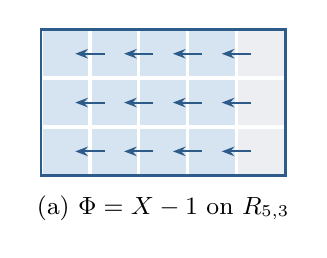
\begin{tikzpicture}[scale=0.62]
 \foreach \i in {0,...,3} \foreach \j in {0,1,2} \fill[nlightblue] (\i,\j) rectangle ++(1,1);
 \foreach \j in {0,1,2} \fill[nlightgray] (4,\j) rectangle ++(1,1);
 \draw[white,line width=1.2pt] (0,0) grid (5,3);
 \draw[nblue,line width=1pt] (0,0) rectangle (5,3);
 \foreach \i in {0,...,3} \foreach \j in {0,1,2}
   \draw[-{Stealth[length=1.6mm]}, nblue, line width=0.7pt] (\i+1.3,\j+0.5) -- (\i+0.7,\j+0.5);
 \node[below] at (2.5,-0.2) {\small (a) $\Phi=X-1$ on $R_{5,3}$};
\end{tikzpicture}
\hspace{1.4cm}
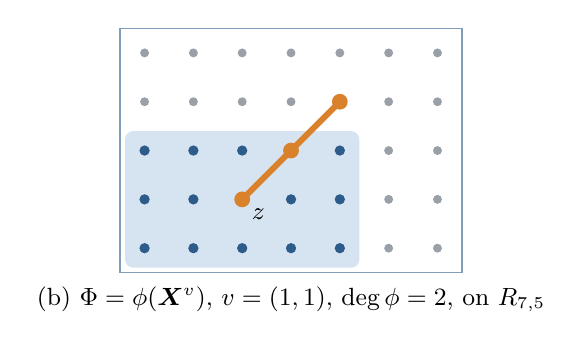
\begin{tikzpicture}[scale=0.62]
 \fill[nlightblue, rounded corners=3pt] (-0.4,-0.4) rectangle (4.4,2.4);
 \foreach \x in {0,...,6} \foreach \y in {0,...,4} \fill[ngray] (\x,\y) circle (2.6pt);
 \foreach \x in {0,...,4} \foreach \y in {0,1,2} \fill[nblue] (\x,\y) circle (3pt);
 \draw[norange, line width=2.2pt, line cap=round] (2,1) -- (4,3);
 \foreach \p in {(2,1),(3,2),(4,3)} \fill[norange] \p circle (4.6pt);
 \node[below right, font=\small] at (2,1) {$z$};
 \draw[nblue!60, line width=0.6pt] (-0.5,-0.5) rectangle (6.5,4.5);
 \node[below] at (3,-0.6) {\small (b) $\Phi=\phi(\mon v)$, $v=(1,1)$, $\deg\phi=2$, on $R_{7,5}$};
\end{tikzpicture}
\caption{The set $S$ of~\eqref{eq:erosion} (blue). (a) For the horizontal difference, $(\Phi(T)c)(z)=c(z+(1,0))-c(z)$ reads the right-hand neighbour of $z$, so $S=R_{4,3}$. (b) For a polynomial in $\mon v$ of degree $2$, $\supp\Phi$ lies in $\{0,v,2v\}$ and contains $0$ and $2v$ (orange, placed at a site $z$ of $S$), so it has widths $w_1=w_2=2$ and $S=R_{5,3}$.}
\label{fig:erosion}
\end{figure}

\begin{proof}
Because $R$ is a product of intervals, $z+\supp\Phi\subseteq R$ holds if and only if $a_j\le z_j+u_j\le b_j$ for all $u\in\supp\Phi$ and $j=1,2$. That is, $a_j\le z_j+\alpha_j$ and $z_j+\beta_j\le b_j$. The remaining assertions follow by counting.
\end{proof}

This is the first place where the rectangular shape of $R$ is used. It guarantees that $S$ is again a rectangle, so that the induction on area can continue. The shape is used again, more essentially, in Lemma~\ref{lem:supported}.

\subsection{The three propositions}
The proof of Theorem~\ref{thm:main} rests on the following three results.

\begin{letterprop}{A}[counting]\label{prop:A}
Let $c$ be a configuration and let $x,y\in X_c$. Suppose that $0\ne\Phi\in\LL$ generates the whole annihilator ideal of their difference:
\[
 \Ann(x-y)=(\Phi).
\]
Let $R$ be a rectangle and define $S$ by~\eqref{eq:erosion}. Then
\[
 P_{\Phi(T)c}(S)-|S|\ \le\ P_c(R)-|R|.
\]
\end{letterprop}

\begin{letterprop}{B}[finding the operator]\label{prop:B}
Let $c$ be a configuration that is not periodic and has a nonzero annihilator. Then there are $x,y\in X_c$ with $x\ne y$, a primitive vector $v$, an integer $q\ge1$, and a monic nonconstant polynomial $\phi\in\Q[Z]$ dividing $Z^q-1$, such that
\[
 \Ann(x-y)=\bigl(\phi(\mon v)\bigr).
\]
\end{letterprop}

\begin{letterprop}{C}[two difference operators]\label{prop:C}
Let $c$ be a configuration with $P_c(m,n)\le mn$ for some $m,n\ge1$. If
\[
 \De_h\De_tc=0
\]
for some nonzero $h,t\in\Z^2$, then $c$ is periodic.
\end{letterprop}

Proposition~\ref{prop:A} is the counting estimate described in the introduction: when $P_c(R)\le|R|$, it gives $P_{\Phi(T)c}(S)\le|S|$. Proposition~\ref{prop:B} supplies an operator to which it applies. Since $\phi(\mon v)$ involves only the monomials $\mon{iv}$, the operator $\Phi(T)=\phi(T^v)$ acts along the single direction $v$. It is also a factor of $\De_{qv}$, because $\De_{qv}=\psi(T^v)\phi(T^v)$ with $\psi=(Z^q-1)/\phi$. Proposition~\ref{prop:C} is what lets us return from $\Phi(T)c$ to $c$.

\subsection{Proof of Nivat's conjecture from the three propositions}
Figure~\ref{fig:flow} summarizes the argument.

\begin{figure}[ht]
\centering
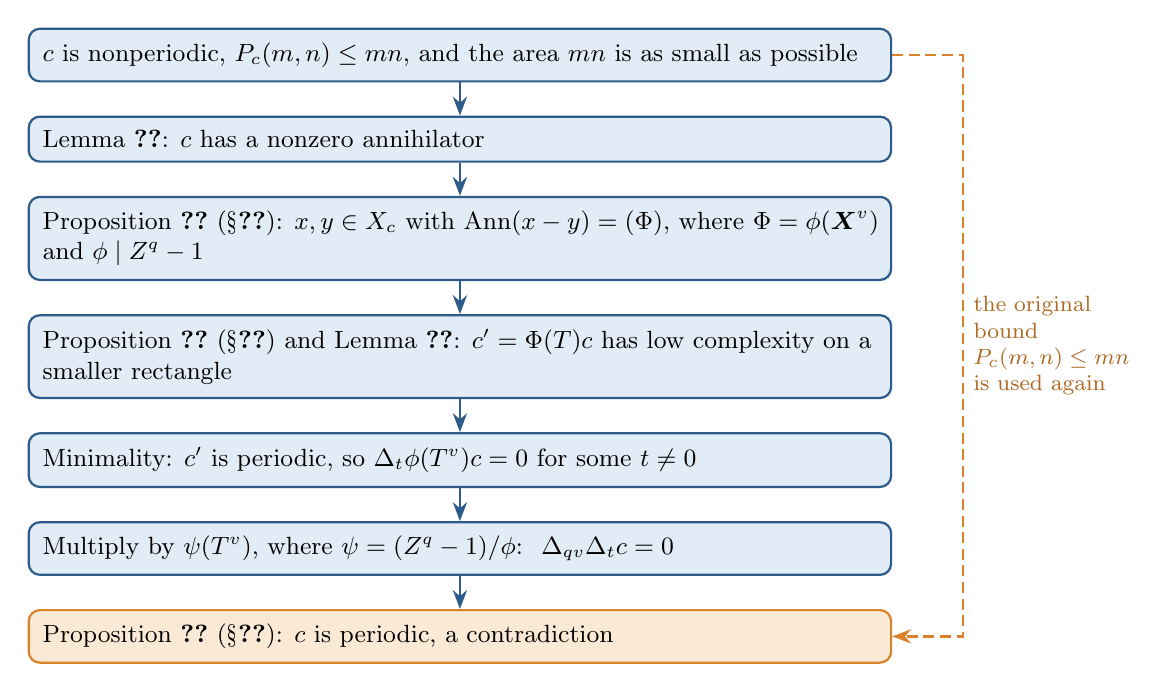
\begin{tikzpicture}[
  box/.style={draw=nblue, fill=nlightblue!70, rounded corners=4pt, text width=10.6cm, align=flush left, inner sep=5pt, font=\small, line width=0.8pt},
  arr/.style={-{Stealth[length=2.4mm]}, line width=0.9pt, nblue},
  node distance=4.2mm]
 \node[box] (a) {$c$ is nonperiodic, $P_c(m,n)\le mn$, and the area $mn$ is as small as possible};
 \node[box, below=of a] (b) {Lemma~\ref{lem:ann-exists}: $c$ has a nonzero annihilator};
 \node[box, below=of b] (c) {Proposition~\ref{prop:B} (\S\ref{sec:filter}): $x,y\in X_c$ with $\Ann(x-y)=(\Phi)$, where $\Phi=\phi(\mon v)$ and $\phi\mid Z^q-1$};
 \node[box, below=of c] (d) {Proposition~\ref{prop:A} (\S\ref{sec:descent}) and Lemma~\ref{lem:erosion}: $c'=\Phi(T)c$ has low complexity on a smaller rectangle};
 \node[box, below=of d] (e) {Minimality: $c'$ is periodic, so $\De_t\phi(T^v)c=0$ for some $t\ne0$};
 \node[box, below=of e] (f) {Multiply by $\psi(T^v)$, where $\psi=(Z^q-1)/\phi$: $\;\De_{qv}\De_tc=0$};
 \node[box, below=of f, draw=norange, fill=nlightorange!80] (g) {Proposition~\ref{prop:C} (\S\ref{sec:twofactor}): $c$ is periodic, a contradiction};
 \foreach \u/\v in {a/b,b/c,c/d,d/e,e/f,f/g} \draw[arr] (\u) -- (\v);
 \draw[arr, norange, dash pattern=on 4pt off 2pt] (a.east) -- ++(0.9,0) |- (g.east)
   node[pos=0.25, right, font=\footnotesize, align=left, text=norange!80!black] {the original\\ bound\\ $P_c(m,n)\le mn$\\ is used again};
\end{tikzpicture}
\caption{The structure of the proof of Theorem~\ref{thm:main}.}
\label{fig:flow}
\end{figure}

\begin{proof}[Proof of Theorem~\ref{thm:main}]
By the rational labelling, it suffices to treat finite-range rational configurations. Suppose the theorem fails. Among all nonperiodic configurations $c$, with any finite set of rational values, and all $m,n$ with $P_c(m,n)\le mn$, choose one for which the area $mn$ is as small as possible. Put $R=R_{m,n}$.

By Lemma~\ref{lem:ann-exists}, $c$ has a nonzero annihilator. Proposition~\ref{prop:B} provides $x,y\in X_c$, a primitive $v$, an integer $q\ge1$, and a monic $\phi$ of degree $\ell\ge1$ dividing $Z^q-1$, with
\[
 \Ann(x-y)=(\Phi),\qquad \Phi=\phi(\mon v)=\sum_{i=0}^{\ell}a_i\mon{iv}.
\]
Here $a_\ell=1$, and $a_0=\phi(0)\ne0$ because $\phi$ divides $Z^q-1$. So $\supp\Phi$ contains $0$ and $\ell v\ne0$, and $\Phi$ is not a monomial.

Let $c'=\Phi(T)c$, again a finite-range rational configuration, and define $S$ by~\eqref{eq:erosion}. Proposition~\ref{prop:A} gives
\[
 P_{c'}(S)\le|S|+P_c(R)-|R|\le|S|.
\]
The set $S$ is not empty, since otherwise this inequality would read $1\le0$. By Lemma~\ref{lem:erosion}, $S$ is a rectangle of area less than $mn$, and since complexity is unchanged by translation, $c'$ satisfies the hypothesis of the theorem on a rectangle of smaller area. By the minimality of $mn$, the configuration $c'$ is periodic. Choose a period $t\ne0$, so that
\[
 \De_t\,\phi(T^v)\,c=0.
\]
Write $Z^q-1=\psi(Z)\phi(Z)$ and apply $\psi(T^v)$. Since the operators commute and $\psi(T^v)\phi(T^v)=T^{qv}-I=\De_{qv}$, we obtain
\[
 \De_{qv}\De_tc=0.
\]
Now Proposition~\ref{prop:C}, applied to $c$ with its original bound $P_c(m,n)\le mn$, shows that $c$ is periodic. This contradiction proves the theorem.
\end{proof}

Three features of this argument deserve comment.
\begin{enumerate}
\item The minimum is taken over configurations with arbitrary finite sets of rational values, because $c'=\Phi(T)c$ generally takes values that $c$ does not.
\item Proposition~\ref{prop:C} is applied to the original configuration $c$ and the original rectangle. The smaller rectangle is used only to make $c'$ periodic.
\item Proposition~\ref{prop:A} holds for any nonzero $\Phi$. The special form $\Phi=\phi(\mon v)$ with $\phi\mid Z^q-1$ is needed only in the last step, to convert the periodicity of $c'$ into the identity $\De_{qv}\De_tc=0$.\footnote{The original paper states the area reduction (its Corollary~2.3) only for polynomials of the form $\phi(\mon v)$. Lemma~\ref{lem:erosion} is the same computation for general $\Phi$. The Lean formalization proves the area reduction in this generality, for every nonzero $\Phi$ annihilating a nonzero configuration.}
\end{enumerate}

\subsection{Sources of the ingredients}
We follow the original paper's account of where the ingredients come from.

The link between few patterns and annihilators is due to Kari and Szabados~\cite{KS}, as is the theorem that a nonzero annihilator can be upgraded to a product of difference operators (Proposition~\ref{prop:product}, proved in Appendix~\ref{app:product}). Cancelling difference operators on configurations that vanish on a half-plane is taken from Kari and Moutot~\cite{KM}. The existence of two limits agreeing on a half-plane is a symbolic consequence of results of Boyle and Lind~\cite{BL} and of Einsiedler, Lind, Miles and Ward~\cite{ELMW}; a direct proof is given in Lemma~\ref{lem:halfplane-pair}.

Proposition~\ref{prop:C} includes Szabados's theorem that Nivat's conjecture holds for sums of two periodic configurations~\cite{Sz} (such sums satisfy its hypothesis; see Section~\ref{sec:twofactor}), and its proof follows his, which in turn uses ideas of Cyr and Kra~\cite{CK}.

Kari and Szabados already relate linear dependence of patterns to polynomial annihilators~\cite[proofs of Lemmas~6 and~32]{KS}. Proposition~\ref{prop:A} applies this relation to differences of patterns that have the same image under $\Phi$. For that estimate, for the computation of the full annihilator ideal in Theorem~\ref{thm:exact-ideal}, and for the induction on area that combines them, the original paper cites no earlier source.

\section{The counting argument: proof of Proposition~\ref{prop:A}}\label{sec:descent}

Write $c'=\Phi(T)c$. We want to show that at least $|R|-|S|$ patterns are lost in passing from $c$ on $R$ to $c'$ on $S$, that is, $P_c(R)-P_{c'}(S)\ge|R|-|S|$. We begin with the simplest case, which already shows why the hypothesis is an \emph{equality} of ideals and not merely the statement that $\Phi$ annihilates $x-y$.

\subsection{A warm-up: horizontal differences}\label{ssec:warmup}
Take $\Phi=X-1$, so that $\Phi(T)=\De_{(1,0)}$, and $R=R_{m,n}$. Then $S=R_{m-1,n}$ (Figure~\ref{fig:erosion}(a)). A pattern on $R$ is a vector $p\in\Q^R$, and applying $\Phi$ turns it into a pattern on $S$ by the linear map
\[
 F\colon\Q^R\to\Q^S,\qquad (Fp)(i,j)=p(i+1,j)-p(i,j).
\]
The kernel of $F$ consists of the patterns that are constant along each row $\{(i,j):0\le i<m\}$ of $R$. It has dimension $n=|R|-|S|$.

Let $\mathcal P=\Pat_c(R)$. The patterns of $c'$ on $S$ are the images $F(p)$ for $p\in\mathcal P$. Group the patterns in $\mathcal P$ into \emph{fibres}, two patterns lying in the same fibre when they have the same image under $F$. Then $P_{c'}(S)$ is the number of fibres. A fibre containing $k$ patterns contributes $k-1$ to the loss $P_c(R)-P_{c'}(S)$, and the differences of its members span a space of dimension at most $k-1$. So
\[
 P_c(R)-P_{c'}(S)\ \ge\ \dim\spanQ\{p-p': p,p'\in\mathcal P,\ Fp=Fp'\}.
\]
All the differences on the right lie in $\ker F$. To get the required drop of $n$, it is enough that they span all of $\ker F$.

Where can we find many pairs of patterns in the same fibre? Suppose that $x,y\in X_c$ and that $d=x-y$ is annihilated by $\Phi$, so that $d(i,j)=g(j)$ depends only on the row. For each site $a$, the patterns of $x$ and $y$ on $R$ at $a$ both belong to $\mathcal P$. They lie in the same fibre, and their difference is the row-constant pattern whose row values are $g(a_2),\ldots,g(a_2+n-1)$. These patterns span $\ker F$ if and only if the vectors
\[
 \bigl(g(b),g(b+1),\ldots,g(b+n-1)\bigr),\qquad b\in\Z,
\]
span $\Q^n$. If $g$ is the indicator function of $\{j\ge0\}$, they do: they include all the ``staircase'' vectors $(0,\ldots,0,1,\ldots,1)$. If $g$ is a nonzero constant, they span only a line, and we learn only that the number of patterns drops by at least one.

The two cases differ in their annihilators. When $g$ is constant, $d$ is also annihilated by $Y-1$, which is supported in $R$ (if $n\ge2$) but is not a multiple of $X-1$. When $g$ is the step function, every annihilator of $d$ is a multiple of $X-1$ (this follows from Theorem~\ref{thm:exact-ideal} below). In general the translates of $d$ span $\ker F$ precisely when every annihilator of $d$ supported in $R$ is a multiple of $\Phi$ (this is Step~2 of Section~\ref{ssec:proofA}). The hypothesis $\Ann(x-y)=(\Phi)$ guarantees this for every rectangle at once.\footnote{The constant-difference comparison in this subsection is not in the original paper, which makes the same point with a shorter remark after its Theorem~2.2.}

\subsection{Multiples of \texorpdfstring{$\Phi$}{Phi} supported in a rectangle}
We identify $\Q^D$, the space of functions $D\to\Q$, with the space of Laurent polynomials supported in $D$, by $p\mapsto\sum_{z\in D}p(z)\mon z$. We need to know which multiples of $\Phi$ lie in $\Q^R$.

\begin{lemma}\label{lem:supported}
Let $R$ be a rectangle, let $0\ne\Phi\in\LL$, and define $S$ by~\eqref{eq:erosion}. Then
\[
 (\Phi)\cap\Q^R=\Phi\cdot\Q^S,
\]
and this space has dimension $|S|$.
\end{lemma}

\begin{proof}
If $g\in\Q^S$, then every monomial of $\Phi g$ has exponent $z+u$ with $z\in S$ and $u\in\supp\Phi$, which lies in $R$. So $\Phi g\in\Q^R$.

Conversely, suppose $g\in\LL$ is nonzero and $\Phi g\in\Q^R$. We use the fact that extreme exponents add under multiplication. Regard $\Phi$ and $g$ as Laurent polynomials in $X$ with coefficients in the integral domain $\Q[Y^{\pm1}]$. The product of their leading coefficients is nonzero, so the largest power of $X$ occurring in $\Phi g$ is the sum of the largest powers occurring in $\Phi$ and in $g$. The same holds for smallest powers and for the variable $Y$. With $[a_j,b_j]$ the coordinate intervals of $R$ and $\alpha_j,\beta_j$ as in Lemma~\ref{lem:erosion}, it follows that every $z\in\supp g$ satisfies $a_j-\alpha_j\le z_j\le b_j-\beta_j$ for $j=1,2$. For instance, the largest power of $X$ in $\Phi g$ is at most $b_1$ and equals $\beta_1$ plus the largest power of $X$ in $g$, so every $z\in\supp g$ has $z_1\le b_1-\beta_1$. By Lemma~\ref{lem:erosion}, this says $z\in S$. Hence $g\in\Q^S$.

Finally, multiplication by $\Phi$ is injective because $\LL$ is an integral domain, so $\Phi\cdot\Q^S$ has dimension $|S|$.
\end{proof}

The rectangular shape of $R$ is essential in the converse direction, where the bounding box of $\supp g$ is compared with $R$. For other windows the lemma can fail. With $\Phi=1-X$ and $g=1+X+Y$, the product $\Phi g=1+Y-X^2-XY$ is supported in the four-point set $R=\{(0,0),(0,1),(1,1),(2,0)\}$. For this $R$ the set $S$ is $\{(0,1)\}$, which does not contain $\supp g$.\footnote{This example is not in the original paper.}

\subsection{Proof of Proposition~\ref{prop:A}}\label{ssec:proofA}
Let $d=x-y$. For finite $D$, equip $\Q^D$ with the standard pairing $\langle p,g\rangle_D=\sum_{z\in D}p(z)g(z)$.

\emph{Step 1: the map on patterns and its kernel.} Write $\Phi=\sum_u\Phi_u\mon u$. Define
\[
 F\colon\Q^R\to\Q^S,\qquad (Fp)(z)=\sum_u\Phi_u\,p(z+u).
\]
This makes sense because $z+u\in R$ whenever $z\in S$ and $u\in\supp\Phi$. The map $F$ computes $\Phi(T)$ locally: for every configuration $e$ and site $a$,
\begin{equation}\label{eq:F-local}
 F\bigl(\restr{(T^ae)}{R}\bigr)=\restr{\bigl(T^a\,\Phi(T)e\bigr)}{S}.
\end{equation}
Its transpose is multiplication by $\Phi$. Indeed, for $p\in\Q^R$ and $g\in\Q^S$,
\[
 \langle Fp,g\rangle_S=\sum_{z\in S}\sum_u g(z)\Phi_u\,p(z+u)=\langle p,\Phi g\rangle_R.
\]
By Lemma~\ref{lem:supported}, the transpose $F^{\mathsf T}\colon g\mapsto\Phi g$ is injective with image $\Phi\cdot\Q^S$. A linear map and its transpose have the same rank, and the kernel of a map is the orthogonal complement of the image of its transpose. So $F$ has rank $|S|$, and
\begin{equation}\label{eq:kernel-dim}
 \dim\ker F=|R|-|S|,\qquad (\ker F)^\perp=\operatorname{im}F^{\mathsf T}=\Phi\cdot\Q^S.
\end{equation}

\emph{Step 2: the translates of $d$ span the kernel.} Let
\[
 V=\spanQ\bigl\{\restr{(T^ad)}{R}: a\in\Z^2\bigr\}\subseteq\Q^R.
\]
A vector $b\in\Q^R$ is orthogonal to $V$ if and only if $\sum_{z\in R}b(z)\,d(a+z)=0$ for every $a$, that is, if and only if the polynomial $b$ annihilates $d$. Using the hypothesis and Lemma~\ref{lem:supported},
\[
 V^\perp=\Ann(d)\cap\Q^R=(\Phi)\cap\Q^R=\Phi\cdot\Q^S=(\ker F)^\perp.
\]
The pairing on $\Q^R$ is nondegenerate, so taking orthogonal complements gives
\begin{equation}\label{eq:full-kernel}
 V=\ker F.
\end{equation}

\emph{Step 3: counting.} Let $\mathcal P=\Pat_c(R)$ and $c'=\Phi(T)c$. By~\eqref{eq:F-local} with $e=c$, the map $F$ sends $\mathcal P$ onto $\Pat_{c'}(S)$. In each fibre of $F|_{\mathcal P}$ choose one pattern, and subtract it from each of the other patterns in the fibre. This produces a list of $P_c(R)-P_{c'}(S)$ vectors spanning the space
\[
 U=\spanQ\{p-p': p,p'\in\mathcal P,\ Fp=Fp'\}.
\]
Since $x,y\in X_c$, the patterns $\restr{(T^ax)}{R}$ and $\restr{(T^ay)}{R}$ belong to $\mathcal P$ for every $a$. By~\eqref{eq:F-local} their images under $F$ differ by $\restr{(T^a\Phi(T)d)}{S}=0$. So their difference $\restr{(T^ad)}{R}$ lies in $U$, and hence $V\subseteq U$. Combining this with~\eqref{eq:full-kernel} and~\eqref{eq:kernel-dim},
\[
 |R|-|S|=\dim V\le\dim U\le P_c(R)-P_{c'}(S),
\]
which is Proposition~\ref{prop:A}.\qed

\begin{example}\label{ex:sharp}
The inequality can be an equality. Let $d(i,j)=1$ if $j\ge i$ and $d(i,j)=0$ otherwise, and let $\Phi=XY-1$. This configuration is invariant under translation by $(1,1)$ and vanishes below the diagonal. Translating $d$ far to the right gives configurations converging to $0$, so $x=d$ and $y=0$ both lie in $X_d$. Theorem~\ref{thm:exact-ideal} below gives $\Ann(d)=(XY-1)$. On $R_{m,n}$ the quantity $j-i$ takes $m+n-1$ consecutive values, and the patterns of $d$ are exactly the $m+n$ threshold patterns $\{j-i\ge s\}$. Since $\Phi(T)d=0$ and $|S|=(m-1)(n-1)$,
\[
 P_d(R)-P_{\Phi(T)d}(S)=m+n-1=|R|-|S|.
\]
\end{example}

\section{Finding the operator: proof of Proposition~\ref{prop:B}}\label{sec:filter}

Let $c$ be a nonperiodic configuration with a nonzero annihilator. We must find $x,y\in X_c$ whose difference has a principal annihilator ideal, generated by a polynomial along one lattice direction. The construction has four steps.
\begin{enumerate}
\item A compactness argument gives $x\ne y$ in $X_c$ that agree on an open half-plane (Section~\ref{ssec:halfplane}). This is the only place where nonperiodicity of $c$ is used.
\item By~\eqref{eq:inheritance}, $d=x-y$ has a nonzero annihilator, and a theorem of Kari and Szabados turns it into a product of difference operators (Section~\ref{ssec:product}).
\item Difference operators transverse to the boundary of the half-plane cannot annihilate $d$, so they can be cancelled. This leaves a period of $d$ parallel to the boundary (Section~\ref{ssec:tangent}).
\item The half-plane is used a second time to show that $d$ satisfies no relation involving the transverse direction beyond those forced by the relations along the boundary. So $\Ann(d)$ is generated by a single polynomial in $\mon v$ (Section~\ref{ssec:exact}).
\end{enumerate}
Figure~\ref{fig:difference} shows the kind of configuration $d$ that this produces.

\begin{figure}[ht]
\centering
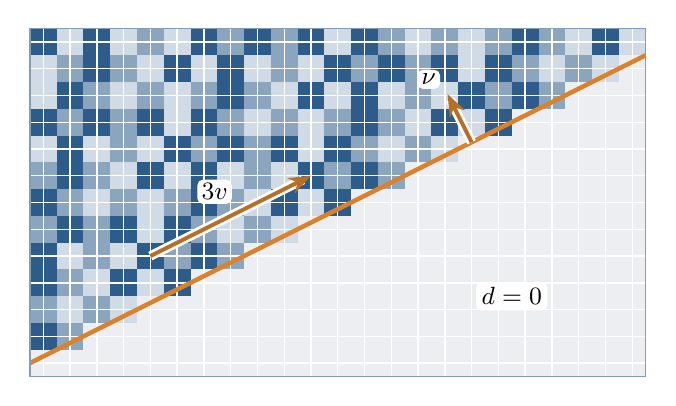
\begin{tikzpicture}[scale=0.34]
 \foreach \x in {-11,...,11}{
  \foreach \y in {-6,...,6}{
   \pgfmathtruncatemacro\b{2*\y-\x}
   \pgfmathtruncatemacro\a{\x-\y}
   \ifnum\b<0
     \fill[nlightgray] (\x-0.5,\y-0.5) rectangle (\x+0.5,\y+0.5);
   \else
     \pgfmathtruncatemacro\val{Mod(\a+Mod(\b*\b*\b+2*\b,7),3)}
     \ifcase\val \def\col{nblue}\or \def\col{nblue!55}\or \def\col{nblue!22}\fi
     \fill[\col] (\x-0.5,\y-0.5) rectangle (\x+0.5,\y+0.5);
   \fi
  }
 }
 \draw[white,line width=0.5pt] (-11.5,-6.5) grid (11.5,6.5);
 \draw[norange, line width=1.6pt] (-11.5,-6) -- (11.5,5.5);
 \draw[white, line width=3.4pt] (-7,-2) -- (-1.3,0.85);
 \draw[-{Stealth[length=2.8mm]}, norange!85!black, line width=1.4pt] (-7,-2) -- (-1,1);
 \node[fill=white, rounded corners=2pt, inner sep=1.5pt, font=\small] at (-4.6,0.4) {$3v$};
 \draw[white, line width=3.4pt] (5,2.25) -- (4.2,3.85);
 \draw[-{Stealth[length=2.8mm]}, norange!85!black, line width=1.4pt] (5,2.25) -- (4.1,4.05);
 \node[fill=white, rounded corners=2pt, inner sep=1.5pt, font=\small] at (3.4,4.6) {$\nu$};
 \node[fill=white, rounded corners=2pt, inner sep=2pt, font=\small] at (6.5,-3.5) {$d=0$};
 \draw[nblue!60, line width=0.6pt] (-11.5,-6.5) rectangle (11.5,6.5);
\end{tikzpicture}
\caption{A configuration of the kind produced in this section, with $v=(2,1)$ and $q=3$. It vanishes (grey) on the half-plane below a line parallel to $v$, and it is invariant under translation by $3v$. The three shades of blue stand for three nonzero values. Nothing constrains how $d$ varies from one row parallel to $v$ to the next.}
\label{fig:difference}
\end{figure}

\begin{heuristic}
The one-dimensional model is a nonzero sequence $(a_k)_{k\in\Z}$ that vanishes for $k<0$. Such a sequence satisfies no linear recurrence $\sum_{j=0}^Jf_ja_{k+j}=0$ ($k\in\Z$) with constant coefficients, except the trivial one. Indeed, if $a_{k_0}$ is its first nonzero term, the relation at $k=k_0-J$ reads $f_Ja_{k_0}=0$, so $f_J=0$, and repeating the argument kills every coefficient. In particular the sequence is not periodic. A configuration vanishing on a half-plane behaves in the same way in the direction transverse to the boundary, with rows playing the role of terms and polynomials in the shift along the rows playing the role of coefficients. Step~(3) uses this to cancel transverse difference operators, and step~(4) uses the ``first nonzero row'' version of the argument above.
\end{heuristic}

\subsection{Two limits that agree on a half-plane}\label{ssec:halfplane}

\begin{lemma}\label{lem:halfplane-pair}
Let $c$ be a configuration with infinitely many distinct translates. Then there are $x,y\in X_c$ and a unit vector $\nu\in\R^2$ such that
\[
 x(0)\ne y(0),\qquad x(z)=y(z)\ \text{ whenever }\ \nu\cdot z<0.
\]
\end{lemma}

The idea is shown in Figure~\ref{fig:halfplane}. Take two translates of $c$ that agree on a large ball, and look at them from a nearest point of disagreement. From that point the ball looks, at close range, like a half-plane.

\begin{figure}[ht]
\centering
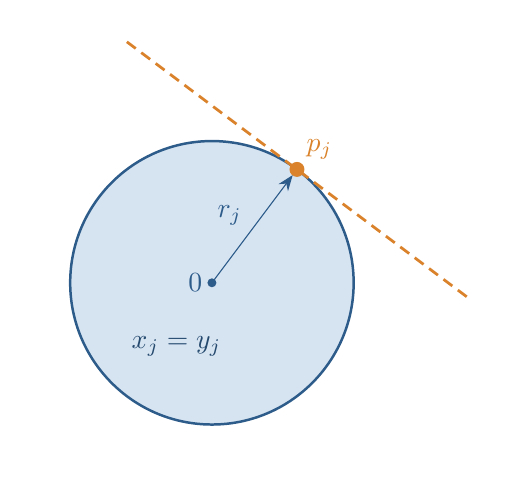
\begin{tikzpicture}[scale=0.9]
 \clip (-2.6,-2.6) rectangle (4.0,3.6);
 \fill[nlightblue] (0,0) circle (2);
 \draw[nblue, line width=0.9pt] (0,0) circle (2);
 \draw[norange, line width=1pt, dash pattern=on 4pt off 2.5pt] (-1.2,3.4) -- (3.6,-0.2);
 \fill[nblue] (0,0) circle (1.8pt) node[left] {$0$};
 \draw[-{Stealth[length=2mm]}, nblue] (0,0) -- (1.14,1.52);
 \node[nblue] at (0.25,0.95) {$r_j$};
 \fill[norange] (1.2,1.6) circle (3pt) node[above right] {$p_j$};
 \node[nblue!80!black] at (-0.5,-0.9) {$x_j=y_j$};
\end{tikzpicture}
\hspace{0.8cm}
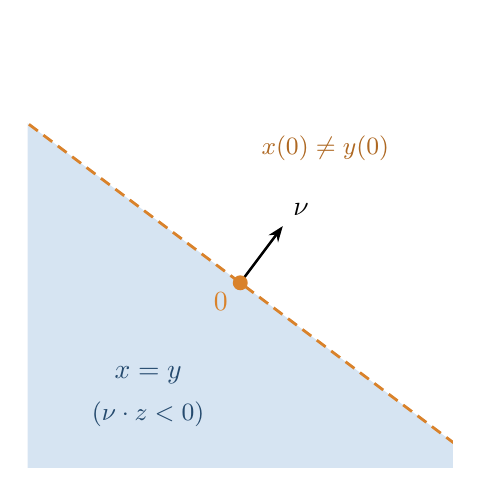
\begin{tikzpicture}[scale=0.9]
 \clip (-3.0,-2.6) rectangle (3.0,3.6);
 \fill[nlightblue] (-4.2,3.15) -- (4.2,-3.15) -- (-4.2,-3.15) -- cycle;
 \draw[norange, line width=1pt, dash pattern=on 4pt off 2.5pt] (-4.2,3.15) -- (4.2,-3.15);
 \draw[-{Stealth[length=2mm]}, line width=0.9pt] (0,0) -- (0.6,0.8) node[above right] {$\nu$};
 \fill[norange] (0,0) circle (3pt) node[below left, xshift=-1pt] {$0$};
 \node[nblue!80!black] at (-1.3,-1.3) {$x=y$};
 \node[nblue!80!black, font=\small] at (-1.3,-1.85) {($\nu\cdot z<0$)};
 \node[norange!80!black, font=\small] at (1.2,1.9) {$x(0)\ne y(0)$};
\end{tikzpicture}
\caption{Left: the translates $x_j,y_j$ agree on the open ball of radius $r_j=\|p_j\|$ (blue) and differ at $p_j$. Near $p_j$ the ball is close to the half-plane bounded by the dashed tangent line. Right: recentring at $p_j$ and passing to a limit gives $x,y$ that agree on an open half-plane and differ at the origin.}
\label{fig:halfplane}
\end{figure}

\begin{proof}
For each positive integer $j$, the ball $\{z:\|z\|\le j\}$ contains finitely many lattice points, so $c$ has only finitely many patterns on it. Since $c$ has infinitely many distinct translates, two of them, $x_j\ne y_j$, have the same pattern on this ball. Let $p_j$ be a site where they differ with $\|p_j\|$ as small as possible. Such a site exists because $\|z\|^2$ takes nonnegative integer values. Put $r_j=\|p_j\|$. Then $r_j>j$, and $x_j,y_j$ agree at every $z$ with $\|z\|<r_j$.

Pass to a subsequence along which $T^{p_j}x_j\to x$ and $T^{p_j}y_j\to y$ pointwise, $p_j/r_j\to\nu$ for some unit vector $\nu$, and the pair of symbols $(x_j(p_j),y_j(p_j))$ is constant. This is possible because the alphabet is finite and the unit circle is compact. Then $x,y\in X_c$, being limits of translates of $c$, and $x(0)\ne y(0)$.

Now fix $z$ with $\nu\cdot z<0$. Then
\[
 \|p_j+z\|^2-r_j^2=2r_j\,\bigl((p_j/r_j)\cdot z\bigr)+\|z\|^2,
\]
which is negative for all large $j$, because $r_j\to\infty$ and $(p_j/r_j)\cdot z\to\nu\cdot z<0$. So $x_j$ and $y_j$ agree at $p_j+z$ for all large $j$, and in the limit $x(z)=y(z)$.
\end{proof}

At this stage the direction $\nu$ is an arbitrary unit vector. Its orthogonal line need not contain any nonzero lattice points. Section~\ref{ssec:tangent} will show that it does.

\subsection{Products of difference operators}\label{ssec:product}
The following theorem of Kari and Szabados~\cite[Theorem~11 and Corollary~12]{KS} converts an arbitrary nonzero annihilator into one of a very special form. A self-contained proof of the version stated here, which allows repeated directions, is given in Appendix~\ref{app:product}. It uses only integer arithmetic and an interpolation identity.

\begin{proposition}[Kari--Szabados]\label{prop:product}
If a nonzero configuration $c$ has a nonzero annihilator, then there are $s\ge1$ and nonzero vectors $h_1,\ldots,h_s\in\Z^2$ with
\[
 \De_{h_1}\cdots\De_{h_s}c=0.
\]
\end{proposition}

We will also need the fact that a repeated difference operator can be reduced to a single one on bounded configurations. For finite-range configurations this is a special case of~\cite[Lemmas~9--10]{KS}.

\begin{lemma}\label{lem:repeated}
Let $e\colon\Z^2\to\Q$ be bounded, let $h\ne0$, and let $s\ge1$. If $\De_h^se=0$, then $\De_he=0$.
\end{lemma}

\begin{proof}
Fix $z$ and consider the bounded sequence $a_k=e(z+kh)$. Suppose $s\ge2$. Its $s$-th difference vanishes, so its $(s-1)$-st difference is a constant $C$. If $C\ne0$, the $(s-2)$-nd difference would grow linearly, which is impossible for a bounded sequence. So $C=0$, and the $(s-1)$-st difference vanishes. Repeating the argument brings us down to $s=1$.
\end{proof}

\subsection{A period along the boundary}\label{ssec:tangent}
The following cancellation argument is due to Kari and Moutot~\cite[Proposition~13 and the proof of Lemma~17]{KM}.

\begin{proposition}\label{prop:tangent-period}
Let $d\ne0$ be a configuration with a nonzero annihilator, and suppose $d(z)=0$ whenever $\nu\cdot z<0$, for some nonzero $\nu\in\R^2$. Then there are a primitive $v\in\Z^2$ with $\nu\cdot v=0$ and an integer $q\ge1$ such that $T^{qv}d=d$.
\end{proposition}

\begin{proof}
Let $\mathcal V$ be the space of rational-valued functions $e$ on $\Z^2$ that vanish on some half-plane $\{z:\nu\cdot z<b\}$, where $b\in\R$ may depend on $e$. Because $b$ is allowed to vary, $\mathcal V$ is preserved by all shifts, and hence by all difference operators.

If $\nu\cdot h\ne0$, then $\De_h$ is injective on $\mathcal V$. Indeed, if $e\in\mathcal V$ and $\De_he=0$, then $e$ is constant along each line $z+\Z h$. Each such line enters the half-plane where $e$ vanishes, because $\nu\cdot(z+kh)\to-\infty$ as $k\to\infty$ or as $k\to-\infty$. So $e=0$.

By Proposition~\ref{prop:product}, $\De_{h_1}\cdots\De_{h_s}d=0$. Order the factors so that the transverse ones, those with $\nu\cdot h_i\ne0$, come first, and let $e$ be the product of the remaining factors applied to $d$. Then $e\in\mathcal V$, and the transverse factors can be cancelled one at a time by injectivity. This gives $e=0$. If no factors remained, this would say $d=0$. So some $h_i$ with $\nu\cdot h_i=0$ exists. In particular the line $\nu^\perp$ contains a nonzero lattice point, so $\nu^\perp\cap\Z^2=\Z v$ for a primitive vector $v$. The remaining factors have the form $h_i=q_iv$ with $q_i\ne0$, and
\[
 \prod_i\bigl(T^{q_iv}-I\bigr)\,d=0.
\]
Let $q\ge1$ be a common multiple of the $|q_i|$. In $\Q[Z^{\pm1}]$ each $Z^{q_i}-1$ divides $Z^q-1$ (for negative $q_i$, note $Z^{q_i}-1=-Z^{q_i}(Z^{|q_i|}-1)$). So if $r$ factors remain, their product divides $(Z^q-1)^r$, and therefore $\De_{qv}^{\,r}d=0$. Since $d$ has finite range, Lemma~\ref{lem:repeated} gives $\De_{qv}d=0$.
\end{proof}

The cancellation happens inside $\mathcal V$. On the space of all configurations, no difference operator is injective. The argument is also specifically two-dimensional: all the surviving directions must lie on the single line $\nu^\perp$.

\subsection{The full annihilator ideal}\label{ssec:exact}
A period $qv$ gives the annihilator $\mon{qv}-1$. Proposition~\ref{prop:A}, however, needs a generator of the \emph{whole} ideal $\Ann(d)$. The next theorem computes that ideal, and the answer involves only the direction $v$.

\begin{theorem}\label{thm:exact-ideal}
Let $d\colon\Z^2\to\Q$ be nonzero, let $v$ be primitive and $q\ge1$, and suppose that $T^{qv}d=d$. Suppose also that $d(z)=0$ whenever $\nu\cdot z<0$, where $\nu\ne0$ and $\nu\cdot v=0$.\footnote{The original paper allows a half-plane whose boundary is any line parallel to $v$. The case of a boundary through the origin is all that the proof of Proposition~\ref{prop:B} needs.} Let $\phi\in\Q[Z]$ be the monic polynomial of least degree with $\phi(T^v)d=0$. Then $\phi$ is nonconstant, $\phi$ divides $Z^q-1$, and
\[
 \Ann(d)=\bigl(\phi(\mon v)\bigr).
\]
\end{theorem}

\begin{figure}[ht]
\centering
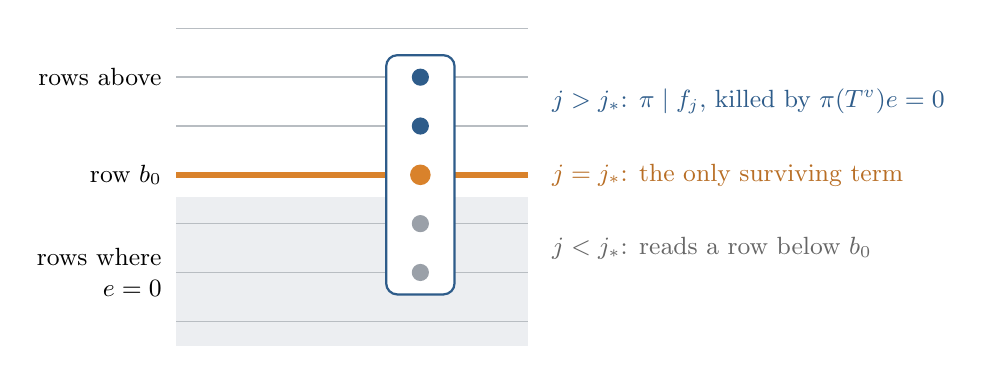
\begin{tikzpicture}[scale=0.62]
 \fill[nlightgray] (-1,-3.5) rectangle (6.2,-0.45);
 \foreach \r in {-3,...,3} \draw[ngray!70, line width=0.5pt] (-1,\r) -- (6.2,\r);
 \draw[norange, line width=2.4pt] (-1,0) -- (6.2,0);
 \node[left, font=\small] at (-1.1,0) {row $b_0$};
 \node[left, font=\small, align=right] at (-1.1,-2) {rows where\\ $e=0$};
 \node[left, font=\small] at (-1.1,2) {rows above};
 \fill[white, rounded corners=4pt, draw=nblue, line width=0.8pt] (3.3,-2.45) rectangle (4.7,2.45);
 \foreach \j in {-2,-1} \fill[ngray] (4,\j) circle (5pt);
 \fill[norange] (4,0) circle (6pt);
 \foreach \j in {1,2} \fill[nblue] (4,\j) circle (5pt);
 \node[right, font=\small, text=nblue, align=left] at (6.5,1.5) {$j>j_*$: $\pi\mid f_j$, killed by $\pi(T^v)e=0$};
 \node[right, font=\small, text=norange!85!black, align=left] at (6.5,0) {$j=j_*$: the only surviving term};
 \node[right, font=\small, text=black!60, align=left] at (6.5,-1.5) {$j<j_*$: reads a row below $b_0$};
\end{tikzpicture}
\caption{The first-row argument in the proof of Theorem~\ref{thm:exact-ideal}, with $j_*=2$. The term $f_j(Z)W^j$ of $G$, evaluated on row $b_0-j_*$, reads row $b_0-j_*+j$ of $e$. Terms above $j_*$ are killed algebraically and terms below it are killed by the half-plane. What remains is a relation on the single row $b_0$.}
\label{fig:firstrow}
\end{figure}

\begin{proof}
\emph{Coordinates.} Complete $v$ to a basis $v,w$ of $\Z^2$, choosing the sign of $w$ so that $\nu\cdot w>0$. For $z=av+bw$ we have $\nu\cdot z=b\,(\nu\cdot w)$, so $d$ vanishes at $av+bw$ whenever $b<0$. We call $\{av+bw:a\in\Z\}$ \emph{row $b$}. The ring isomorphism $\LL\to\Q[Z^{\pm1},W^{\pm1}]$ sending $\mon{av+bw}$ to $Z^aW^b$ is compatible with the action on configurations, with $Z$ acting by $T^v$ and $W$ by $T^w$. We work in the new variables. Note that a polynomial in $Z$ alone acts separately on each row.

\emph{The polynomial along rows.} The polynomials $g\in\Q[Z]$ with $g(T^v)d=0$ form an ideal of $\Q[Z]$, and it contains $Z^q-1$. Its monic generator is $\phi$, which therefore divides $Z^q-1$. It is nonconstant because $d\ne0$. The polynomial $Z^q-1$ is squarefree, because it is coprime to its derivative $qZ^{q-1}$. Hence $\phi$ is squarefree. Every multiple of $\phi(Z)$ in $\Q[Z^{\pm1},W^{\pm1}]$ annihilates $d$. It remains to prove the converse.

\emph{Every annihilator is a multiple of $\phi$.} Let $G$ annihilate $d$. After multiplying by a monomial, which is a unit, we may assume $G$ is an ordinary polynomial, $G=\sum_{j\ge0}f_j(Z)W^j$. Let $\pi$ be an irreducible factor of $\phi$ in $\Q[Z]$. We claim that $\pi$ divides every coefficient $f_j$. Suppose not; we shall reach a contradiction. Let
\[
 e=(\phi/\pi)(T^v)\,d.
\]
Then $e\ne0$, because $\phi/\pi$ has smaller degree than $\phi$, and $\phi$ has the least degree among polynomials in $Z$ annihilating $d$. Also $e$ vanishes on rows $b<0$, since $(\phi/\pi)(T^v)$ acts within rows. Moreover $\pi(T^v)e=\phi(T^v)d=0$ and $G(T)e=(\phi/\pi)(T^v)G(T)d=0$, since the operators commute.

Let $j_*$ be the largest index with $\pi\nmid f_{j_*}$, and let $b_0$ be the lowest nonzero row of $e$. It exists because $e\ne0$ and $e$ vanishes on all negative rows. Evaluate $G(T)e=0$ on row $b_0-j_*$ (Figure~\ref{fig:firstrow}). Here $(G(T)e)(av+(b_0-j_*)w)=\sum_j\bigl(f_j(T^v)e\bigr)(av+(b_0-j_*+j)w)$. For $j>j_*$ the term vanishes because $f_j$ is a multiple of $\pi$ and $\pi(T^v)e=0$. For $j<j_*$ it vanishes because it only involves row $b_0-j_*+j$, which lies below $b_0$ and where $e$ is zero. What remains says that the sequence $u(a)=e(av+b_0w)$, which is row $b_0$ of $e$ and is not identically zero, satisfies
\[
 f_{j_*}(\sigma)u=0\qquad\text{and}\qquad \pi(\sigma)u=0,
\]
where $\sigma$ is the shift on sequences. Since $\pi$ is irreducible and does not divide $f_{j_*}$, Bézout's identity gives $A,B\in\Q[Z]$ with $A\pi+Bf_{j_*}=1$. Applying this to $u$ gives $u=0$, a contradiction.

So each irreducible factor $\pi$ of $\phi$ divides every $f_j$, hence divides $G$ in $\Q[Z,W]$. The irreducible factors of $\phi$ are pairwise non-associate, because $\phi$ is squarefree, and they remain prime in $\Q[Z,W]$, because $\Q[Z,W]/(\pi)\cong(\Q[Z]/(\pi))[W]$ is a polynomial ring over a field. Therefore their product $\phi$ divides $G$. Undoing the monomial factor and the change of variables proves the theorem.
\end{proof}

The theorem uses the \emph{minimal} polynomial $\phi$, not the period polynomial $Z^q-1$. This choice is forced. For $d(i,j)=1$ if $j\ge0$ and $0$ otherwise, the theorem gives $\Ann(d)=(X-1)$, although $X^2-1$ also annihilates $d$. On an $m\times n$ rectangle with $m\ge2$, the translates of $d$ span a space of dimension $n$, while the kernel of the map induced by $X^2-1$ has dimension $2n$. With $X^2-1$ in place of $X-1$, the equality~\eqref{eq:full-kernel} would fail.

\subsection{Proof of Proposition~\ref{prop:B}}
Let $c$ be nonperiodic with a nonzero annihilator. If two translates $T^uc$ and $T^{u'}c$ with $u\ne u'$ were equal, then $u-u'$ would be a period. So $c$ has infinitely many distinct translates, and Lemma~\ref{lem:halfplane-pair} provides $x,y\in X_c$ and a unit vector $\nu$ such that $d=x-y$ is nonzero and vanishes on $\{\nu\cdot z<0\}$. The configuration $d$ has finite range, since $x$ and $y$ take values in $c(\Z^2)$, and it has a nonzero annihilator by~\eqref{eq:inheritance}. Proposition~\ref{prop:tangent-period} gives a primitive $v$ with $\nu\cdot v=0$ and $q\ge1$ with $T^{qv}d=d$. Theorem~\ref{thm:exact-ideal} then gives $\Ann(d)=(\phi(\mon v))$ with $\phi$ monic, nonconstant, and dividing $Z^q-1$.\qed

\section{Two difference operators: proof of Proposition~\ref{prop:C}}\label{sec:twofactor}

This section proves Proposition~\ref{prop:C}. The argument follows Szabados's proof that Nivat's conjecture holds for sums of two periodic configurations~\cite{Sz}. It uses his boundary selection, his count of ambiguous extensions, and his finite description of strips; the source of each is indicated below. One step differs from~\cite{Sz}. Szabados extends periodicity from a strip using a general strip-extension result~\cite[Lemma~3 and Appendix~A.2]{Sz}. Here the identity $\De_h\De_tc=0$ and a finite recurrence are used instead (Lemma~\ref{lem:row-lifting}). Apart from Lemma~\ref{lem:repeated}, this section uses nothing from Sections~\ref{sec:descent} and~\ref{sec:filter}.

\subsection{What the hypothesis says, and the parallel case}
The identity $\De_h\De_tc=0$ can be read in two ways: $\De_tc$ is $h$-periodic, and $\De_hc$ is $t$-periodic. For example, if $c=a+b$ where $a$ is $t$-periodic and $b$ is $h$-periodic, then $\De_tc=\De_tb$ is $h$-periodic. Such sums need not be periodic, as $c(i,j)=f(i)+g(j)$ with $f$ and $g$ nonperiodic finite-range sequences shows. So the complexity hypothesis must be used.

When $h$ and $t$ are parallel, however, complexity is not needed.

\begin{lemma}\label{lem:parallel}
If $h,t$ are nonzero and parallel and $\De_h\De_tc=0$, then $c$ is periodic.
\end{lemma}

\begin{proof}
Replacing $t$ by $-t$ preserves the hypothesis, because $\De_{-t}=-T^{-t}\De_t$. Since $h$ and $t$ are parallel lattice vectors, we may therefore assume that they point the same way, and then they have a common multiple $u=\alpha h=\beta t$ with integers $\alpha,\beta\ge1$. Then
\[
 \De_u=\Bigl(\sum_{i<\alpha}T^{ih}\Bigr)\De_h=\Bigl(\sum_{i<\beta}T^{it}\Bigr)\De_t,
\]
so $\De_u^2c$ is a product of commuting operators applied to $\De_h\De_tc=0$. Lemma~\ref{lem:repeated} gives $\De_uc=0$.
\end{proof}

\subsection{Coordinates, and the plan for the nonparallel case}\label{ssec:plan}
From now on $h$ and $t$ are not parallel. Write $h=qv$ with $v$ primitive and $q\ge1$, and complete $v$ to a basis $v,w$ of $\Z^2$ (the sign of $w$ will be fixed in Lemma~\ref{lem:boundary-window}). We write
\[
 \rc ij=iv+jw,
\]
call $\{\rc ij:i\in\Z\}$ \emph{row $j$}, and order each row by $i$. These are not the standard coordinates, and a rectangle in $\Z^2$ is generally not a rectangle in these coordinates. We say that row $j$ of a configuration $x$ is \emph{periodic} if $x(\rc{i+p}j)=x(\rc ij)$ for all $i$ and some $p\ge1$.

Since $t$ is not parallel to $v$, we have $t=\rc aM$ with $M\ne0$. Replacing $t$ by $-t$ if necessary (which preserves the hypothesis, as in Lemma~\ref{lem:parallel}), we will arrange $M\ge1$. Two consequences of the hypothesis drive the argument.
\begin{enumerate}
\item[(O1)] \emph{Finitely many rows suffice.} Suppose $p$ is a positive multiple of $q$ and $\De_{pv}c$ vanishes on $M$ consecutive rows. Then $\De_{pv}c$ is $t$-periodic, because $\De_{pv}=\bigl(\sum_{i<p/q}T^{iqv}\bigr)\De_h$ and $\De_hc$ is $t$-periodic. Translation by $t$ moves each site up $M$ rows, so every $t$-orbit meets those $M$ rows. Hence $\De_{pv}c=0$, and $pv$ is a period (Figure~\ref{fig:O1}).
\item[(O2)] \emph{Translates along $t$ differ periodically.} For all $j,k$, the difference $T^{jt}c-T^{kt}c$ is a sum of translates of $\De_tc$, hence is $h$-periodic.
\end{enumerate}
\begin{figure}[ht]
\centering
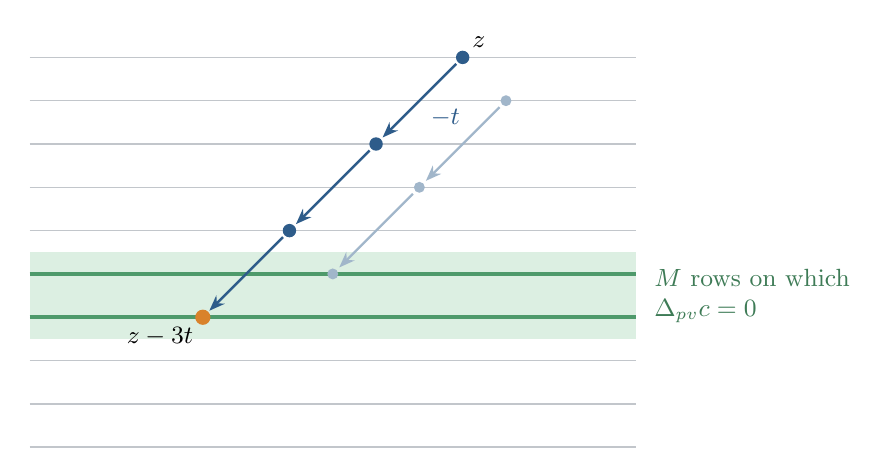
\begin{tikzpicture}[scale=0.55]
 \fill[nlightgreen] (-7,1.5) rectangle (7,3.5);
 \foreach \j in {-1,...,8} \draw[ngray!60, line width=0.5pt] (-7,\j) -- (7,\j);
 \foreach \j in {2,3} \draw[ngreen, line width=1.4pt] (-7,\j) -- (7,\j);
 \node[right, font=\small, text=ngreen!80!black, align=left] at (7.2,2.5) {$M$ rows on which\\ $\De_{pv}c=0$};
 \foreach \s/\x/\y in {0/3/8,1/1/6,2/-1/4,3/-3/2} \fill[nblue] (\x,\y) circle (4.4pt);
 \foreach \x/\y in {3/8,1/6,-1/4} \draw[-{Stealth[length=2mm]}, nblue, line width=0.9pt] (\x-0.15,\y-0.15) -- (\x-1.85,\y-1.85);
 \node[nblue, font=\small] at (2.6,6.6) {$-t$};
 \node[above right, font=\small] at (3,8) {$z$};
 \fill[norange] (-3,2) circle (5pt);
 \node[below left, font=\small] at (-3,2) {$z-3t$};
 \foreach \s/\x/\y in {0/4/7,1/2/5,2/0/3} \fill[nblue!45] (\x,\y) circle (3.6pt);
 \foreach \x/\y in {4/7,2/5} \draw[-{Stealth[length=2mm]}, nblue!45, line width=0.8pt] (\x-0.15,\y-0.15) -- (\x-1.85,\y-1.85);
\end{tikzpicture}
\caption{Observation~(O1) with $t=\rc2 2$ and $M=2$. Since $\De_{pv}c$ is $t$-periodic, its value at any site $z$ equals its value at $z-nt$ for all $n$. Each step moves down $M$ rows, so every $t$-orbit meets any band of $M$ consecutive rows. If $\De_{pv}c$ vanishes on one such band (green), it vanishes everywhere.}
\label{fig:O1}
\end{figure}

Observation~(O1) matters because individual periodicity of rows does not give a common period in general. The configuration $c(i,j)=1$ if $i\equiv0\pmod{|j|+2}$ and $0$ otherwise has every row periodic but no nonzero horizontal period. Under our hypothesis it suffices to make finitely many rows periodic, and finitely many periods have a common multiple.

The proof has four steps.
\begin{enumerate}
\item \emph{A boundary rule} (Lemma~\ref{lem:boundary-window}). From $P_c(m,n)\le mn$ we extract a finite window $B$ with bottom row $E$ and upper part $C=B\setminus E$, and a local rule: the values of $c$ on $C$ together with a few sites of $E$ determine the value at the next site of $E$.
\item \emph{A strip pair} (Lemma~\ref{lem:strip-states}). Using~(O2), either some multiple of $t$ is a period of $c$, or there are two translates $x,y$ of $c$ that agree on a strip of rows $1,\ldots,W$, with $W$ at least the number of rows of $C$, but differ somewhere on row $0$, with $x-y$ being $h$-periodic.
\item \emph{Periodic rows above the boundary} (Lemma~\ref{lem:periodic-interior}). If $x$ and $y$ agreed on a whole copy of $E$ in row $0$, the boundary rule would propagate agreement rightward along row $0$, and $h$-periodicity of $x-y$ would then force agreement on all of row $0$. So $x$ and $y$ disagree on every copy of $E$ in row $0$. Consequently every $C$-pattern of $x$ along the strip has two different extensions to $B$. Few patterns have this property, and Morse--Hedlund makes the rows of the strip periodic.
\item \emph{Spreading periodicity} (Lemma~\ref{lem:row-lifting}). With the rows above periodic, the boundary rule becomes a finite-memory recurrence with periodic input, so the next row down is periodic too. After finitely many rows, (O1) applies.
\end{enumerate}

\subsection{One-dimensional tools}
The three results below all say that a sequence is periodic when each term determines the next. The first is the basic form, where a single term determines its successor.

\begin{lemma}\label{lem:finite-states}
Let $s\colon\Z\to\Sigma$ be a sequence with finite range such that $s_i=s_j$ implies $s_{i+1}=s_{j+1}$. Then $s$ has a period $p$ with $1\le p\le|s(\Z)|$. The same holds if instead $s_i=s_j$ implies $s_{i-1}=s_{j-1}$.
\end{lemma}

\begin{proof}
The hypothesis says that $\tau(s_i)=s_{i+1}$ defines a map $\tau$ on the finite set $s(\Z)$. It is surjective, since $s_i=\tau(s_{i-1})$, and hence bijective. Therefore $s_i=\tau^i(s_0)$ for all $i\in\Z$ (for negative $i$, use $\tau^{-1}$), and $s$ has period equal to the length of the cycle of $\tau$ through $s_0$. The second version follows by reversing the indices.
\end{proof}

\begin{corollary}[Morse--Hedlund]\label{cor:morse}
If a bi-infinite word with finite range has at most $n$ distinct subwords of length $n$, where $n\ge1$, then it has a period $p$ with $1\le p\le n$.
\end{corollary}

For completeness we include the usual extension-count proof; compare~\cite[Section~2.1]{CK}.

\begin{proof}
Let $N(j)$ be the number of distinct subwords of length $j$, so $N(0)=1$. Every subword extends to the right, so $N$ is nondecreasing. If $N(j+1)>N(j)$ for every $0\le j<n$, then $N(n)\ge n+1$. So $N(j+1)=N(j)$ for some $0\le j<n$. Then every subword of length $j$ has exactly one extension by one letter on the right. Consider the sequence whose $i$-th term is the subword of length $j+1$ starting at position $i$. If two terms are equal, their last $j$ letters are equal, so the next letters are equal too, and so are the next terms. This sequence takes $N(j+1)\le N(n)\le n$ values, so by Lemma~\ref{lem:finite-states} it has a period at most $n$, which is also a period of the word.
\end{proof}

The last tool allows an external input. In words: if each term of $a$ is determined by the previous $k$ terms together with the current value of a periodic sequence $\eta$, then $a$ is periodic. The hypothesis compares only values that actually occur in $a$ and $\eta$; nothing is assumed about other inputs.

\begin{lemma}\label{lem:forcing}
Let $a\colon\Z\to\Q$ have finite range and let $\eta\colon\Z\to\Sigma$ be periodic. Suppose that for some $k\ge0$ and all $i,i'$:
\[
 \eta_i=\eta_{i'}\ \text{ and }\ a_{i+\ell}=a_{i'+\ell}\ (0\le\ell<k)\quad\Longrightarrow\quad a_{i+k}=a_{i'+k}.
\]
Then $a$ is periodic.
\end{lemma}

\begin{proof}
Let $p\ge1$ be a period of $\eta$ and consider the states $s_i=(i\bmod p,\,a_i,a_{i+1},\ldots,a_{i+k})$, which take finitely many values. If $s_i=s_{i'}$, then $\eta_{i+1}=\eta_{i'+1}$ and $a_{i+1+\ell}=a_{i'+1+\ell}$ for $\ell<k$, so the hypothesis at $i+1,i'+1$ gives $a_{i+1+k}=a_{i'+1+k}$, and hence $s_{i+1}=s_{i'+1}$. Lemma~\ref{lem:finite-states} applies.
\end{proof}

The period of $a$ need not be related to the period of $\eta$. For example, with $\eta$ constant, the recurrence $a_{i+1}=1-a_i$ has solutions of period two. For this reason we combine periods only at the end, by taking common multiples of finitely many periods.

\subsection{A boundary row with a unique-extension rule}\label{ssec:window}
Imagine building $R$ up from the empty set one site at a time. There is $P_c(\varnothing)=1$ pattern at the start and at most $|R|$ at the end, so on average each site adds fewer than one new pattern. We make this precise row by row. We remove the rows of $R$ one at a time, keeping track of the difference between the number of patterns and the number of sites, and stop at the first step where this difference becomes positive. At that step the removed row had added fewer new patterns than it has sites. Then, adding the sites of that row back one at a time, some site adds no new pattern at all: its value is determined by the values already present. This gives a local rule.

To measure the balance, define the \emph{discrepancy} of a finite window $D$ as
\[
 \delta_c(D)=P_c(D)-|D|,
\]
following~\cite[Section~2.2]{CK}. The construction below is a variant of Szabados's edge-removal construction~\cite[Lemma~2]{Sz}, combined with the unique-extension step from the proof of~\cite[Lemma~4]{Sz}. The row-length estimate uses the interpolation argument of~\cite[Lemma~2.11]{CK}. We always remove the shorter of the two extreme rows, so that the remaining rows stay long. That length is needed in step~(3) of the plan.

\begin{lemma}\label{lem:boundary-window}
Let $R$ be a rectangle with $P_c(R)\le|R|$, and let $v$ be primitive. Then, for a suitable choice of the sign of $w$, there are integers $e\ge1$, $H\ge0$ and $0\le k<e$, and a finite set $B$ that is a translate of a subset of $R$, with the following properties.
\begin{enumerate}
\item $B$ lies in rows $0,\ldots,H$. Its part in row $0$ is $E=\{\rc00,\rc10,\ldots,\rc{e-1}0\}$, and its part in each row is a set of consecutive sites. For $0\le j\le H$, row $j$ of $B$ contains at least $e-1$ sites.
\item With $C=B\setminus E$, we have
\[
 P_c(B)\le|B|\qquad\text{and}\qquad r:=P_c(B)-P_c(C)<e.
\]
\item \emph{(Boundary rule.)} Let $D_k=C\cup\{\rc00,\ldots,\rc{k-1}0\}$. For all $u,u'\in\Z^2$,
\[
 \restr{(T^uc)}{D_k}=\restr{(T^{u'}c)}{D_k}\quad\Longrightarrow\quad c(u+\rc k0)=c(u'+\rc k0).
\]
\end{enumerate}
\end{lemma}

\begin{figure}[ht]
\centering
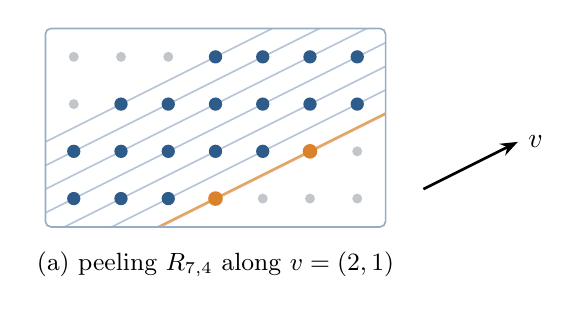
\begin{tikzpicture}[scale=0.6]
 \begin{scope}
  \clip (-0.6,-0.6) rectangle (6.6,3.6);
  \foreach \b in {-2,...,3} \draw[nblue!35, line width=0.6pt] (-2,{(\b-2)/2}) -- (8,{(\b+8)/2});
  \draw[norange!70, line width=1pt] (-2,-2.5) -- (8,2.5);
 \end{scope}
 \foreach \x in {0,...,6}{
  \foreach \y in {0,...,3}{
   \pgfmathtruncatemacro\b{2*\y-\x}
   \ifnum\b<-3 \fill[ngray!60] (\x,\y) circle (3pt);
   \else\ifnum\b>3 \fill[ngray!60] (\x,\y) circle (3pt);
   \else\ifnum\b=-3 \fill[norange] (\x,\y) circle (4.4pt);
   \else \fill[nblue] (\x,\y) circle (4pt);
   \fi\fi\fi
  }
 }
 \draw[nblue!50, line width=0.6pt, rounded corners=2pt] (-0.6,-0.6) rectangle (6.6,3.6);
 \draw[-{Stealth[length=2.2mm]}, line width=1pt] (7.4,0.2) -- (9.4,1.2) node[right] {$v$};
 \node[font=\small] at (3,-1.4) {(a) peeling $R_{7,4}$ along $v=(2,1)$};
\end{tikzpicture}
\hspace{1cm}
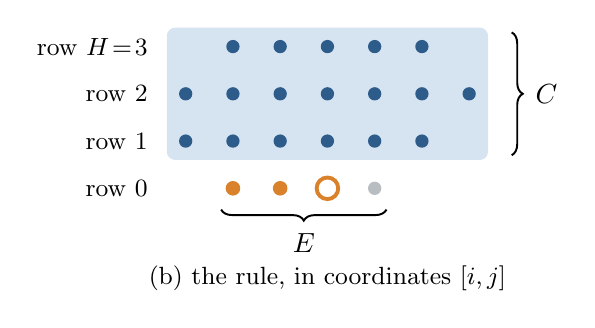
\begin{tikzpicture}[scale=0.6]
 \fill[nlightblue, rounded corners=3pt] (-1.4,0.6) rectangle (5.4,3.4);
 \foreach \i in {-1,...,4} \fill[nblue] (\i,1) circle (4pt);
 \foreach \i in {-1,...,5} \fill[nblue] (\i,2) circle (4pt);
 \foreach \i in {0,...,4} \fill[nblue] (\i,3) circle (4pt);
 \fill[norange] (0,0) circle (4.4pt);
 \fill[norange] (1,0) circle (4.4pt);
 \draw[norange, line width=1.4pt] (2,0) circle (6.5pt);
 \fill[ngray!70] (3,0) circle (4pt);
 \draw[decorate,decoration={brace,mirror,amplitude=4pt}, line width=0.7pt] (-0.25,-0.45) -- (3.25,-0.45) node[midway,below=5pt] {$E$};
 \draw[decorate,decoration={brace,amplitude=4pt}, line width=0.7pt] (5.9,3.3) -- (5.9,0.7) node[midway,right=5pt] {$C$};
 \node[left, font=\small] at (-1.6,0) {row $0$};
 \node[left, font=\small] at (-1.6,1) {row $1$};
 \node[left, font=\small] at (-1.6,2) {row $2$};
 \node[left, font=\small] at (-1.6,3) {row $H\!=\!3$};
 \node[font=\small] at (2,-1.9) {(b) the rule, in coordinates $\rc ij$};
\end{tikzpicture}
\caption{(a) The rows of $R_{7,4}$ for $v=(2,1)$ are the lattice points on lines parallel to $v$. Peeling off the shorter extreme row at each step, with suitable choices in case of ties, removes the grey rows. If the balance first fails at the next step, the blue and orange points form the window $B$ of the lemma, and the orange row, which is removed next, is $E$, with $e=2$. (b) A schematic boundary window with $e=4$, drawn with $v$ horizontal and $w$ vertical. If $k=2$, the values on $D_2=C\cup\{\rc00,\rc10\}$ (blue and orange dots) determine the value at the circled site $\rc20$.}
\label{fig:window}
\end{figure}

\begin{proof}
\emph{Removing rows.} The rows of $R$ in the $(v,w)$ coordinates are its intersections with the lines $\{\rc ij:i\in\R\}$. Starting from $R$, repeatedly delete whichever of the two extreme nonempty rows (the lowest and the highest) has fewer sites, choosing either in case of a tie, until nothing is left. Each set obtained along the way consists of the lattice points in a convex set $K$: the real rectangle spanned by $R$, intersected with a closed strip between two lines parallel to $v$. So each of its rows is a set of consecutive sites: row $j$ of $K$ is a segment, and the lattice points on the line through row $j$ are exactly the points $\rc ij$ with $i\in\Z$, because $v,w$ is a basis of $\Z^2$.

\emph{Row lengths.} Consider a stage of this process whose extreme rows are $j_-<j_+$, occupying the sites $i\in[\alpha_-,\beta_-]$ and $i\in[\alpha_+,\beta_+]$ respectively, and suppose the shorter one has $e$ sites. Then $\beta_\pm-\alpha_\pm\ge e-1$. For $j_-<j<j_+$, write $\lambda=(j-j_-)/(j_+-j_-)$. By convexity, $K$ contains the real points $\rc ij$ with $i$ between $(1-\lambda)\alpha_-+\lambda\alpha_+$ and $(1-\lambda)\beta_-+\lambda\beta_+$. This is an interval of length at least $e-1$, so it contains at least $e-1$ integers. Hence every row between $j_-$ and $j_+$ contains at least $e-1$ sites.

\emph{The first failure of balance.} The discrepancy starts at $\delta_c(R)\le0$ and ends at $\delta_c(\varnothing)=1$. Consider the first deletion step at which it becomes positive, and write it as $B\to C=B\setminus E$, where $E$ is the deleted row and has $e\ge1$ sites. Then $\delta_c(B)\le0$, which is $P_c(B)\le|B|$, and
\[
 0<\delta_c(C)-\delta_c(B)=e-\bigl(P_c(B)-P_c(C)\bigr),
\]
which is $r<e$. Choose the sign of $w$ so that $E$ is the lowest row of $B$, and translate so that $E$ starts at the origin. The other extreme row has at least $e$ sites, since $E$ was the shorter one, so part~(1) follows from the row-length bound.

\emph{The rule.} For $0\le i\le e$, let $D_i=C\cup\{\rc00,\ldots,\rc{i-1}0\}$, so $D_0=C$ and $D_e=B$. The $e$ increments $P_c(D_{i+1})-P_c(D_i)$ are nonnegative integers with sum $r<e$, so one of them, say the $k$-th, is zero. Then restriction from $\Pat_c(D_{k+1})$ to $\Pat_c(D_k)$, which is always surjective, is a bijection between sets of the same size: each pattern on $D_k$ has exactly one extension to the site $\rc k0$. This is part~(3).
\end{proof}

The bound in~(1) is $e-1$ and not $e$, because the endpoints of the interpolated intervals need not be integers. The set $\{\rc00,\rc10,\rc11,\rc12,\rc22\}$ shows this: its extreme rows have two sites each and its middle row has one. When $e=1$, part~(1) says nothing, and middle rows may even be empty. This case is harmless, because Lemma~\ref{lem:periodic-interior} will show that it cannot occur together with a strip pair.\footnote{The original paper leaves this degenerate case implicit.}

Part~(3) is a statement about the set of patterns of $c$, so it holds with $c$ replaced by any translate of $c$.

\subsection{Two translates that agree on a strip}
The next lemma is step~(2) of the plan. By~(O2), the translates $T^{jt}c$ differ from one another by $h$-periodic configurations. So their restrictions to a strip of rows are determined by finitely much data, as in~\cite[Section~6]{Sz}.

\begin{lemma}\label{lem:strip-states}
Suppose $t=\rc aM$ with $M\ge1$ and $\De_h\De_tc=0$, and let $W\ge M$. Then either some nonzero multiple of $t$ is a period of $c$, or there are translates $x,y$ of $c$ such that $x-y$ is $h$-periodic, $x=y$ on rows $1,\ldots,W$, and $x\ne y$ somewhere on row $0$.
\end{lemma}

\begin{proof}
Let $S_W$ be the union of rows $1,\ldots,W$, and let $\sigma_j$ be the restriction of $T^{jt}c$ to $S_W$. By~(O2), $T^{jt}c-T^{kt}c$ is $qv$-periodic. So it vanishes on $S_W$ as soon as it vanishes on the finite set $\{\rc i\ell:0\le i<q,\ 1\le\ell\le W\}$. Hence $\sigma_j$ is determined by finitely many values, and the sequence $(\sigma_j)_{j\in\Z}$ takes only finitely many values. (The individual $\sigma_j$ need not be $qv$-periodic.)

Suppose first that $\sigma_j=\sigma_k$ always implies $\sigma_{j-1}=\sigma_{k-1}$. By Lemma~\ref{lem:finite-states}, $(\sigma_j)$ has a period $p\ge1$. Then $T^{pt}c$ and $c$ agree on $S_W+jt$ for every $j$. These sets are the rows $jM+1,\ldots,jM+W$, and since $W\ge M$ they cover $\Z^2$. So $pt$ is a period of $c$.

Otherwise, choose $j,k$ with $\sigma_j=\sigma_k$ and $\sigma_{j-1}\ne\sigma_{k-1}$. The translates $x_0=T^{jt}c$ and $y_0=T^{kt}c$ agree on rows $1,\ldots,W$ and differ somewhere on $S_W-t$, which consists of rows $1-M,\ldots,W-M$. They agree on the positive rows among these, so they differ on some row in $\{1-M,\ldots,0\}$. Let $s$ be the highest such row, and put $x=T^{sw}x_0$ and $y=T^{sw}y_0$, so that row $j$ of $x$ is row $s+j$ of $x_0$. Then $x$ and $y$ differ on row $0$. Their rows $1,\ldots,W$ are rows $s+1,\ldots,s+W$ of $x_0$ and $y_0$. The rows up to $0$ agree by the choice of $s$, and the rest lie among rows $1,\ldots,W$ because $s\le0$. Finally, $x-y$ is a translate of $x_0-y_0$ and hence $h$-periodic.
\end{proof}

\subsection{Periodic rows above the boundary}
Now we carry out step~(3) of the plan, following the extension-counting argument of Cyr and Kra~\cite[Lemma~2.24]{CK} as used by Szabados~\cite[Lemma~4]{Sz}. Treating the rows of the strip together as a single word over a product alphabet turns a bound on the number of extensions into a bound on word complexity.

\begin{figure}[ht]
\centering
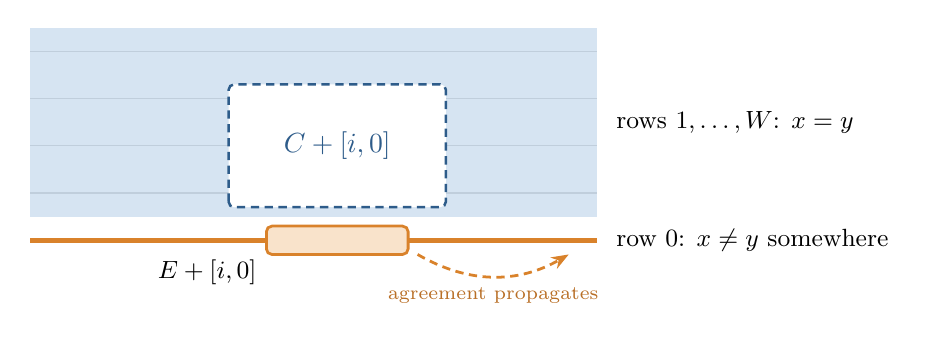
\begin{tikzpicture}[scale=0.6]
 \fill[nlightblue] (-6,0.5) rectangle (6,4.5);
 \foreach \j in {1,...,4} \draw[nblue!30, line width=0.5pt] (-6,\j) -- (6,\j);
 \draw[norange, line width=1.8pt] (-6,0) -- (6,0);
 \fill[white, draw=nblue, line width=0.9pt, dash pattern=on 3pt off 2pt, rounded corners=2pt] (-1.8,0.7) rectangle (2.8,3.3);
 \node[nblue] at (0.5,2) {$C+\rc i0$};
 \fill[nlightorange, draw=norange, line width=1pt, rounded corners=2pt] (-1,-0.3) rectangle (2,0.3);
 \node[below left, font=\small] at (-1,-0.2) {$E+\rc i0$};
 \draw[-{Stealth[length=2.2mm]}, norange, line width=1pt, dash pattern=on 3pt off 2pt] (2.2,-0.3) to[bend right=30] node[below, font=\scriptsize, text=norange!85!black] {agreement propagates} (5.4,-0.3);
 \node[right, font=\small] at (6.2,0) {row $0$: $x\ne y$ somewhere};
 \node[right, font=\small] at (6.2,2.5) {rows $1,\ldots,W$: $x=y$};
\end{tikzpicture}
\caption{Step~(3). The translates $x$ and $y$ agree on the shaded rows and $x-y$ is $qv$-periodic. If they agreed on some copy $E+\rc i0$ of the bottom row, the boundary rule would propagate agreement to the right along row $0$, and periodicity would then give agreement on all of row $0$.}
\label{fig:strip}
\end{figure}

\begin{lemma}\label{lem:periodic-interior}
Let $B,E,C,e,H,k,r$ be as in Lemma~\ref{lem:boundary-window}, with $H\ge1$. Let $x,y$ be translates of $c$ such that $x-y$ is $qv$-periodic, $x=y$ on rows $1,\ldots,H$, and $x\ne y$ somewhere on row $0$. Then $r\ge1$, and there is a $p$ with $1\le p\le r$ such that each of the rows $1,\ldots,H$ of $x$ has period $p$.
\end{lemma}

\begin{proof}
\emph{Step 1: disagreement on every copy of $E$.} We claim that for each $i_0$, the configurations $x$ and $y$ differ somewhere on $E+\rc{i_0}0$. Suppose instead that they agree there. We show by induction on $i$ that they agree at $\rc i0$ for every $i\ge i_0$. For $i<i_0+e$ this is the assumption. For $i\ge i_0+e$, let $u=\rc{i-k}0$. The window $u+D_k$ consists of $C+u$, which lies in rows $1,\ldots,H$ where $x=y$, together with the sites $\rc{i-k}0,\ldots,\rc{i-1}0$, where $x=y$ by induction because $i-k>i_0$. So $x$ and $y$ have the same pattern on $u+D_k$. Since $x$ and $y$ are translates of $c$, the boundary rule applies, and $x(\rc i0)=y(\rc i0)$. Thus $x-y$ vanishes on row $0$ from $i_0$ onwards. Being $qv$-periodic, it then vanishes on all of row $0$, which contradicts the hypothesis.

\emph{Step 2: counting ambiguous patterns.} Call a pattern on $C$ \emph{ambiguous} if it has at least two extensions in $\Pat_c(B)$. Restriction $\Pat_c(B)\to\Pat_c(C)$ is surjective, so the number of ambiguous patterns is at most
\[
 \sum_{p\in\Pat_c(C)}\bigl(\#\{\text{extensions of }p\}-1\bigr)=P_c(B)-P_c(C)=r.
\]
For each $i$, the patterns of $x$ and $y$ on $B$ at $\rc i0$ both occur in $c$. By Step~1 they differ, and they agree on $C$ because $x=y$ on rows $1,\ldots,H$. So the pattern of $x$ on $C$ at $\rc i0$ is ambiguous. There are therefore at most $r$ distinct patterns $\restr{(T^{\rc i0}x)}{C}$, $i\in\Z$, and there is at least one. So $r\ge1$, and hence $e\ge r+1\ge2$.

\emph{Step 3: Morse--Hedlund.} Since $e\ge2$, part~(1) of Lemma~\ref{lem:boundary-window} says that each row $j\in\{1,\ldots,H\}$ of $C$ is a nonempty set of at least $e-1\ge r$ consecutive sites. Let $\rc{\alpha_j}j$ be its first site. Define a word $b$ over a product alphabet by
\[
 b_i=\bigl(x(\rc{\alpha_j+i}j)\bigr)_{j=1}^{H},\qquad i\in\Z.
\]
The subword $b_i,\ldots,b_{i+r-1}$ is read from the sites $\rc{\alpha_j+i+\ell}j$ with $0\le\ell<r$, which form a subset of $C+\rc i0$. So it is determined by the pattern of $x$ on $C$ at $\rc i0$, and $b$ has at most $r$ subwords of length $r$. By Corollary~\ref{cor:morse}, $b$ has a period $p\le r$, and each coordinate of $b$ shows that row $j$ of $x$ has period $p$.
\end{proof}

Only a forward rule was needed. Agreement propagates along a half-row, and the periodic difference then extends it to the whole row. This is where the hypothesis $\De_h\De_tc=0$ enters the counting.

\subsection{Spreading periodicity to the whole plane}
The last step pushes periodicity down one row at a time, then applies~(O1).

\begin{lemma}\label{lem:row-lifting}
Let $h=qv$ and $t=\rc aM$ with $M\ge1$, and suppose $\De_h\De_tx=0$. Suppose that $x$ satisfies the boundary rule of Lemma~\ref{lem:boundary-window}(3) with $H\ge1$, and that each of the rows $1,\ldots,H$ of $x$ is periodic. Then some positive multiple of $h$ is a period of $x$.
\end{lemma}

\begin{proof}
\emph{One row down.} Suppose that rows $j+1,\ldots,j+H$ of $x$ are periodic. We show that row $j$ is periodic. Put
\[
 a_i=x(\rc ij),\qquad \eta_i=\restr{\bigl(T^{\rc ij}x\bigr)}{C}.
\]
Since $C$ lies in rows $1,\ldots,H$, the pattern $\eta_i$ reads only rows $j+1,\ldots,j+H$, and a common period of those rows is a period of $\eta$. The window $\rc ij+D_k$ consists of the sites read by $\eta_i$ together with $\rc ij,\ldots,\rc{i+k-1}j$. So the boundary rule says that $\eta_i$ and $a_i,\ldots,a_{i+k-1}$ determine $a_{i+k}$. By Lemma~\ref{lem:forcing}, row $j$ is periodic.

\emph{Finitely many rows.} Starting from rows $1,\ldots,H$ and working downwards, we obtain $M$ consecutive periodic rows (if $H\ge M$ there is nothing to do). Let $p$ be a common multiple of $q$ and of the periods of these $M$ rows. Then $\De_{pv}x$ vanishes on these rows. By~(O1), applied to $x$, $pv$ is a period of $x$, and it is a positive multiple of $h$.
\end{proof}

\subsection{Proof of Proposition~\ref{prop:C}}
If $h$ and $t$ are parallel, Lemma~\ref{lem:parallel} applies. Otherwise, set up the coordinates of Section~\ref{ssec:plan}, and apply Lemma~\ref{lem:boundary-window} to the rectangle $R_{m,n}$ to obtain $B$ and the sign of $w$. Then $t=\rc aM$ with $M\ne0$. If $M<0$, replace $t$ by $-t$, which preserves the hypothesis and the set of multiples of $t$.

\emph{Case $H=0$.} Then $B=E$ is a single row, and $P_c(E)\le e$. The subwords of length $e$ of any row of $c$ are patterns of $c$ on translates of $E$, so each row has at most $e$ of them. By Corollary~\ref{cor:morse} every row has a period at most $e$, hence a period dividing $e!$. So $e!\,v$ is a period of every row, and $e!\,h=q\,e!\,v$ is a period of $c$.

\emph{Case $H\ge1$.} Let $W=\max(H,M)$. By Lemma~\ref{lem:strip-states}, either a nonzero multiple of $t$ is a period of $c$, or there are translates $x,y$ of $c$ as in that lemma. In the second case, Lemma~\ref{lem:periodic-interior} shows that rows $1,\ldots,H$ of $x$ are periodic. The translate $x$ satisfies $\De_h\De_tx=0$ and the boundary rule, so Lemma~\ref{lem:row-lifting} gives $x$ a period that is a multiple of $h$. A period of a translate of $c$ is a period of $c$.\qed

\medskip
The proof gives slightly more: when $h$ and $t$ are not parallel, some nonzero integer multiple of $h$ or of $t$ is a period of~$c$.

\appendix

\section{Proof of Proposition~\ref{prop:product}}\label{app:product}

The arithmetic step below is Lemma~7 of Kari and Szabados~\cite{KS}, and the resulting product is the one in their Theorem~11. Their Lemma~8 uses the dilation relations in a Vandermonde argument at common zeros. Following the original paper, we instead carry out the corresponding elimination directly in $\LL$.

The idea is as follows. If $f$ annihilates an integer configuration, then so does its ``dilation'' $f_n$, obtained by multiplying all exponents by $n$, for many $n$. This holds because of the Frobenius congruence $f^p\equiv f_p$ modulo a prime $p$. A suitable linear combination of these dilations then eliminates all but one monomial and leaves a product of difference operators.

\begin{proof}[Proof of Proposition~\ref{prop:product}]
Multiplying $c$ and a nonzero annihilator by suitable integers, we may assume both have integer values and coefficients. Write the annihilator as
\[
 f=\sum_{i=0}^{k-1}a_i\mon{u_i}
\]
with distinct $u_i$ and nonzero integers $a_i$. Since $c\ne0$ and a monomial acts invertibly, $k\ge2$. For $n\ge1$ let $f_n=\sum_ia_i\mon{nu_i}$, and let
\[
 K=\max_z|c(z)|\cdot\sum_i|a_i|.
\]
Then every value of every $f_n(T)c$ has absolute value at most $K$.

\emph{Dilations.} Suppose $f_n$ annihilates $c$ and $p>K$ is prime. Modulo $p$, the Frobenius congruence $(y_1+\cdots+y_k)^p\equiv y_1^p+\cdots+y_k^p$ (which follows from the case of two summands, since $\binom pi$ is divisible by $p$ for $0<i<p$) and Fermat's little theorem give $f_n^{\,p}\equiv\sum_ia_i^p\mon{pnu_i}\equiv f_{np}$. So $f_{np}=f_n^{\,p}+p\,g$ for some integer Laurent polynomial $g$, and
\[
 f_{np}(T)c=f_n^{\,p-1}(T)\,f_n(T)c+p\,g(T)c=p\,g(T)c.
\]
Every value of $f_{np}(T)c$ is therefore divisible by $p$ and has absolute value at most $K<p$, so it is zero. Let $\rho=K!$. Every $n\ge1$ coprime to $\rho$ is a product of primes greater than $K$, so starting from $f_1=f$ and applying the previous step once for each prime factor, we get $f_n\in\Ann(c)$ for all such $n$. In particular,
\[
 f_{1+j\rho}\in\Ann(c)\qquad(j\ge0).
\]

\emph{Elimination.} Put $M_i=\mon{\rho u_i}$, so that $f_{1+j\rho}=\sum_ia_i\mon{u_i}M_i^j$. As $j$ varies, these relations form a combination of the geometric sequences $j\mapsto M_i^j$. As in the theory of linear recurrences, combining consecutive terms with the coefficients of a polynomial that vanishes at $M_1,\ldots,M_{k-1}$ cancels all of these sequences except the one with $i=0$. Concretely, expand
\[
 L(U)=\prod_{i=1}^{k-1}(U-M_i)=\sum_{j=0}^{k-1}L_jU^j,\qquad L_j\in\LL.
\]
Then
\[
 \sum_{j=0}^{k-1}L_j\,f_{1+j\rho}=\sum_{i=0}^{k-1}a_i\mon{u_i}L(M_i)=a_0\mon{u_0}\prod_{i=1}^{k-1}(M_0-M_i),
\]
because $L(M_i)=0$ for $i\ge1$. The left side lies in $\Ann(c)$. On the right, $a_0\mon{u_0}$ is a unit, and $M_0-M_i=-M_0\bigl(\mon{\rho(u_i-u_0)}-1\bigr)$. Removing units leaves
\[
 \prod_{i=1}^{k-1}\bigl(\mon{\rho(u_i-u_0)}-1\bigr)\in\Ann(c),
\]
which is a product of difference operators $\De_{\rho(u_i-u_0)}$ with nonzero vectors, because the $u_i$ are distinct.
\end{proof}

For a trinomial $f=\alpha+\beta X+\gamma Y$ (with $u_0=0$), the elimination identity reads
\[
 f_{1+2\rho}-(X^\rho+Y^\rho)f_{1+\rho}+X^\rho Y^\rho f_1=\alpha\,(1-X^\rho)(1-Y^\rho).
\]
The directions in the resulting product may repeat or be parallel. Proposition~\ref{prop:tangent-period} does not need them to be separated, since Lemma~\ref{lem:repeated} removes repetitions after the transverse factors have been cancelled.

\section{Correspondence with the original paper and the Lean formalization}\label{app:map}

The table lists, for each result in this document, the corresponding statement in \emph{Pattern complexity and Nivat's conjecture} (paper/nivat.tex) and the main Lean declarations proving it. Lean names are given with their full namespaces. See also docs/SOURCE\_MAP.md in the repository.

{\small
\begin{longtable}{@{}>{\raggedright\arraybackslash}p{0.2\textwidth}>{\raggedright\arraybackslash}p{0.17\textwidth}>{\raggedright\arraybackslash}p{0.55\textwidth}@{}}
\toprule
This document & Original paper & Lean declaration(s)\\
\midrule
\endhead
Theorem~\ref{thm:main} & Theorem~1.1 & \lean{Nivat.nivat}, \lean{Nivat.nivat_rational}; statement also in \lean{Challenge.lean}\\
Rational labelling & Section~1.1 & \lean{Nivat.exists_rational_model}\\
Inheritance~\eqref{eq:inheritance} & (1.1) & \lean{Nivat.Dynamics.act_eq_zero_of_origin_language}\\
Lemma~\ref{lem:ann-exists} & Lemma~3.2 & \lean{Nivat.Algebra.exists_affine_annihilator}, \lean{Nivat.Algebra.exists_nonzero_annihilator}\\
Lemma~\ref{lem:erosion} & in Lemma~2.1, Corollary~2.3 & \lean{Nivat.Algebra.exists_smaller_rectangle_of_annihilator}\\
Proposition~\ref{prop:A} & Theorem~2.2 & \lean{Nivat.Descent.exact_complexity_descent}; with area reduction: \lean{Nivat.Descent.exists_smaller_low_complexity_rectangle}\\
Lemma~\ref{lem:supported} & Lemma~2.1 & \lean{Nivat.Algebra.support_mul_subset_rectangle_iff}, \lean{Nivat.Descent.multiplierMap_injective}\\
Proof of Prop.~\ref{prop:A}, Steps 1--3 & proof of Theorem~2.2 & \lean{Nivat.Descent.localFilter_transpose}, \lean{Nivat.Descent.translatedSpan_eq_ker}, \lean{Nivat.Descent.finite_fiber_budget}\\
Proposition~\ref{prop:B} & Corollary~3.6 with Theorem~4.1 & \lean{Nivat.Dynamics.periodic_difference_of_nonzero_annihilator} and \lean{Nivat.Algebra.exact_line_in_basis}, combined in \lean{Nivat.nivat_rational}\\
Proposition~\ref{prop:C} & Theorem~5.1 & \lean{Nivat.two_factors}, \lean{Nivat.two_factors_nonparallel}\\
Final step of \S2.5 & Section~6 & \lean{Nivat.periodic_of_periodic_line_filter}\\
Lemma~\ref{lem:halfplane-pair} & Lemma~3.1 & \lean{Nivat.Dynamics.exists_halfPlane_pair}\\
Proposition~\ref{prop:product} & Proposition~3.3, Appendix~A & \lean{Nivat.Algebra.exists_product_differences_of_annihilator}\\
Lemma~\ref{lem:repeated} & Lemma~3.4 & \lean{Nivat.difference_eq_zero_of_iterate_of_bounded}\\
Proposition~\ref{prop:tangent-period} & Proposition~3.5 & \lean{Nivat.Dynamics.exists_tangent_period_of_nonzero_annihilator}\\
Theorem~\ref{thm:exact-ideal} & Theorem~4.1 & \lean{Nivat.Algebra.exact_horizontal_line}, \lean{Nivat.Algebra.exact_line_in_basis}\\
Lemma~\ref{lem:parallel} & proof of Theorem~5.1 & \lean{Nivat.periodic_of_parallel_mixed_difference}\\
Lemma~\ref{lem:finite-states} & Lemma~5.2 & \lean{Nivat.TwoFactors.periodic_of_deterministic_successor_bounded}, \lean{Nivat.TwoFactors.periodic_of_deterministic_predecessor_bounded}\\
Corollary~\ref{cor:morse} & Corollary~5.3 & \lean{Nivat.TwoFactors.morse_hedlund}\\
Lemma~\ref{lem:forcing} & Lemma~5.4 & \lean{Nivat.TwoFactors.periodic_of_periodic_forcing}\\
Lemma~\ref{lem:boundary-window} & Lemma~5.5 & \lean{Nivat.TwoFactors.exists_shapeWindow}, \lean{Nivat.TwoFactors.ShapeWindow.normalize}, \lean{Nivat.TwoFactors.boundaryRule_of_small_cost}\\
Lemma~\ref{lem:strip-states} & Lemma~5.6 & \lean{Nivat.TwoFactors.finite_strip_dichotomy}\\
Lemma~\ref{lem:periodic-interior} & Lemma~5.7 & \lean{Nivat.TwoFactors.every_edge_differs}, \lean{Nivat.TwoFactors.innerOrbit_budget}, \lean{Nivat.TwoFactors.common_inner_period}\\
Lemma~\ref{lem:row-lifting} & Lemma~5.8 & \lean{Nivat.TwoFactors.periodic_of_rows_boundaryRule}\\
\bottomrule
\end{longtable}
}

\begin{thebibliography}{ELMW}
\bibitem[BL]{BL}
M.~Boyle and D.~Lind,
\emph{Expansive subdynamics},
Trans. Amer. Math. Soc. \textbf{349} (1997), no.~1, 55--102.

\bibitem[CK]{CK}
V.~Cyr and B.~Kra,
\emph{Nonexpansive $\mathbb Z^2$-subdynamics and Nivat's conjecture},
Trans. Amer. Math. Soc. \textbf{367} (2015), no.~9, 6487--6537.
Numbering refers to arXiv:1208.4090v2 (2013).

\bibitem[ELMW]{ELMW}
M.~Einsiedler, D.~Lind, R.~Miles, and T.~Ward,
\emph{Expansive subdynamics for algebraic $\mathbb Z^d$-actions},
Ergodic Theory Dynam. Systems \textbf{21} (2001), no.~6, 1695--1729.

\bibitem[GPT]{GPT}
GPT-6 Pro,
\emph{Pattern complexity and Nivat's conjecture}, 14 September 2026.
\url{https://github.com/boonsuan/nivat}.

\bibitem[KM]{KM}
J.~Kari and E.~Moutot,
\emph{Decidability and periodicity of low complexity tilings},
Theory Comput. Syst. \textbf{67} (2023), 125--148.

\bibitem[KS]{KS}
J.~Kari and M.~Szabados,
\emph{An algebraic geometric approach to Nivat's conjecture},
Inform. and Comput. \textbf{271} (2020), article 104481.
Numbering refers to arXiv:1605.05929v1 (2016).

\bibitem[MH]{MH}
M.~Morse and G.~A.~Hedlund,
\emph{Symbolic dynamics},
Amer. J. Math. \textbf{60} (1938), no.~4, 815--866.

\bibitem[Sz]{Sz}
M.~Szabados,
\emph{Nivat's conjecture holds for sums of two periodic configurations},
in \emph{SOFSEM 2018: Theory and Practice of Computer Science},
Lecture Notes in Comput. Sci., vol.~10706, Springer, Cham, 2018, pp.~539--551.
Numbering refers to arXiv:1710.05360v1 (2017).
\end{thebibliography}

\end{document}
